\documentclass[12pt,a4paper,oneside]{article}
%UPISATI JEZIK NA KOJEM JE NAPISAN RAD: HR ili EN
\def\jezik{HR}
\usepackage{lineno, blindtext}
\usepackage{gensymb}

%UPIŠITE: DA ili NE
\def\dvostraniIspis{NE}

%POSTAVKE _setup.tex MORAJU BITI U ISTOJ MAPI GDJE JE I OVAJ DOKUMENT
%\usepackage{showframe} % pokaži marigine

% za brojanje
\usepackage[page,figure,table]{totalcount}

% prored: 1.5
\usepackage{setspace} 
\onehalfspacing

% omogućeni svi hr-znakovi
\usepackage[T1]{fontenc}
\usepackage[utf8]{inputenc}

% tekst-font: Times New Roman 12pt
\usepackage{times}
% promjena veličine fonta
\newcommand{\prored}[1]{\number\numexpr(#1*123)/100\relax}
\newcommand{\velicina}[2][22]{\fontfamily{ptm}\fontsize{#1 pt}{\prored{#1}pt}\selectfont#2}%\sffamily


% OSTALI POTREBNI PAKETI

%za pisanje formula
\usepackage{relsize}
\usepackage{amsmath,mathtools,amsfonts,amssymb,braket}
\usepackage{aurical,calrsfs} %kaligrafija \mathcal{}, \pazocal{}
\numberwithin{equation}{section}

%za liste
\usepackage{enumitem}

%za slike
\usepackage{graphicx,wrapfig,sidecap}
\usepackage[labelfont=bf,textfont={it},font=small]{caption}
\usepackage{pgf,tikz,pgfplots}
%\pgfplotsset{compat=1.11}
\usetikzlibrary{decorations.markings}
\usetikzlibrary{arrows,positioning,shadows}


% za tablice s više redova i definirane širine
\usepackage{multirow,array,colortbl,booktabs}
%\setlength\extrarowheight{3pt}
\newcommand{\urediTablicu}{\centering \fontsize{11pt}{17pt}\selectfont} % font 11pt, 17pt udaljene linije
\setlength{\arrayrulewidth}{0.75pt} % linije debljine 3/4 pt
\newcommand{\hlineRub}{\specialrule{1.5pt}{0pt}{0pt}} %debela horizontalna linija
\newcolumntype{?}{!{\vrule width 1.5pt}} %debela vertikalna linija



% float-naslovi
%\addtolength{\abovecaptionskip}{-3pt}
%\addtolength{\belowcaptionskip}{3pt}

%paketi koji omogućuju korištenje boja
\usepackage{color, xcolor}

%za isticanje i sakrivanje teksta
\usepackage{ulem}
\usepackage{comment}

%za pisanje veb adresa
\usepackage{url}
\urlstyle{same}
%\usepackage{hyperref} %otkomentirati za klikabilne linkove

%za lakšu usporedbu stilova
\usepackage{xstring}
\usepackage{ifthen}

% PRIJEVODI
%zamjena engleskih naziva s njihovim prijevodom
\ifthenelse{\equal{\jezik}{HR}}{
	\renewcommand\refname{\thesection~~~Literatura}
	%\renewcommand{\bibname}{Literatura}
	\renewcommand{\contentsname}{Sadr\v{z}aj}
	\renewcommand{\listfigurename}{Popis slika}
	\renewcommand{\listtablename}{Popis tablica}
	%\renewcommand{\abstractname}{Sa\v{z}etak}
	\renewcommand{\figurename}{Slika}
	\renewcommand{\tablename}{Tablica}
}{
	\renewcommand\refname{\thesection~~~Bibliography}
}

% POSTAVKE STRANICA

%zaglavlja
\usepackage{fancyhdr}
\fancyhf{} %uklanja defaultno zaglavlje/podnožje
\renewcommand{\headrulewidth}{0pt} % uklanja horizontalne crte
\fancyfoot[R]{\thepage}

% marigine
\usepackage[top=2.5cm, left=2.5cm, bottom=2.5cm, right=2.5cm]{geometry}

% dots in ToC
\usepackage{tocloft}
\renewcommand{\cftsecleader}{\cftdotfill{\cftdotsep}}

%uvlačenje paragrafa i razmak između
\setlength{\parindent}{0.4cm}
\setlength{\parskip}{6pt}


%POMOĆNE FUNKCIJE
%za računanje
\usepackage[nomessages]{fp}
\usepackage{calc}
%pomoći brojači za reference i stranice
\newcounter{brRef}\setcounter{brRef}{0}
\newcounter{brStr}\setcounter{brStr}{0}
%provjera postojanosti zahvale
\newlength{\duljinaZahvale}
%provjera postojanosti neposrednog voditelja
\newlength{\duljinaVoditelj}
\newlength{\dTabA}
\newlength{\dTabB}
%dijeljenje modulo
\newcommand{\modulo}[2]{%
	\FPeval{\rezModulo}{trunc(#1-(#2*trunc(#1/#2,0)),0)}%
}
\newcommand{\prijelom}[2]{%
	\ifthenelse{\equal{#1}{DA}\AND\equal{#2}{0}}%
	{~ \newpage}{}%
}
%vraća zadnju znamenku
\newcommand{\jed}[1]{\number\numexpr#1-10*((#1-5)/10)\relax}
%vraća zadnje dvije znamenke
\newcommand{\desJed}[1]{\number\numexpr#1-100*((#1-50)/100)\relax}
%sufiks za stranica, tablica, slika
\newcommand{\padez}[2]{%
	\ifthenelse{\equal{#2}{11}\OR\equal{#2}{12}\OR\equal{#2}{13}\OR\equal{#2}{14}}
		{a}%
		{\ifthenelse{\equal{#1}{2}\OR\equal{#1}{3}\OR\equal{#1}{4}}%
			{e}{\ifthenelse{\equal{#1}{1}}{u}{a}}}}
%sufiks za literaturni navod
\newcommand{\padezRef}[2]{%
	\ifthenelse{\equal{#1}{1}}%
		{literaturni navod}%
		{\ifthenelse{\equal{#2}{11}\OR\equal{#2}{12}\OR\equal{#2}{13}\OR\equal{#2}{14}}%
			{literaturnih navoda}%
			{\ifthenelse{\equal{#1}{2}\OR\equal{#1}{3}\OR\equal{#1}{4}}%
				{literaturna navoda}%
				{literaturnih navoda}}}}


% GENERATORI STRANICA
\newcommand{\kojiRad}{
	\ifthenelse{\equal{\vrstaRada}{1}}{
		\newcommand{\radHR}{Završni rad}
		\newcommand{\radEN}{Bachelor thesis}
	}{
		\newcommand{\radHR}{Diplomski rad}
		\newcommand{\radEN}{Master thesis}
	}
}

\newcommand{\naslovnica}{
	\pagestyle{empty} % bez br. str. 
	\kojiRad
	\begin{titlepage}
		\begin{center}
			\ifthenelse{\equal{\jezik}{HR}}{
				{\velicina[18]{Sveu\v{c}ili\v{s}te u Splitu\\
					Prirodoslovno – matemati\v{c}ki fakultet\\}}
				\vspace{\stretch{6}}
				{\velicina{\textbf{\naslovHR\\}}}
				\vspace{24pt}
				{\velicina[20]{\radHR\\}}
			}{
				{\velicina[18]{University of Split\\
					Faculty of Science\\}}
				\vspace{\stretch{6}}
				{\velicina{\textbf{\naslovEN\\}}}
				\vspace{24pt}
				{\velicina[20]{\radEN\\}}
			}
			\vspace{\stretch{4}}
			{\velicina{\student\\}}
			\vspace{\stretch{11}}
			{\velicina[14]{\mjestoVrijeme\\}}
		\end{center}
	\end{titlepage}
	\setcounter{brStr}{\arabic{page}}
	\stepcounter{brStr}
	\modulo{\thebrStr}{2}
	\prijelom{\dvostraniIspis}{\rezModulo}
	\pagestyle{fancy}
	\pagenumbering{roman}
}

\newcommand{\zahvale}{%
	\StrLen{\zahvala}[\duljinaZahvale]%duljina zahvale
	\ifthenelse{\equal{\duljinaZahvale}{0}}{}{
		\modulo{\arabic{page}}{2}
		\prijelom{\dvostraniIspis}{\rezModulo}
		\zahvala
		\newpage
		\modulo{\arabic{page}}{2}
		\prijelom{\dvostraniIspis}{\rezModulo}}{}
}

\newcommand{\stvoriTabove}{
	\StrLen{\neposredniVoditeljHR}[\duljinaVoditelj]
	\ifthenelse{\equal{\duljinaVoditelj}{0}}{
		\setlength{\dTabA}{3.0cm}
		\setlength{\dTabB}{12.7cm}
	}{
		\setlength{\dTabA}{3.5cm}
		\setlength{\dTabB}{12.2cm}
	}
}

\newcommand{\tdkHR}{
	\modulo{\arabic{page}}{2}
	\prijelom{\dvostraniIspis}{\rezModulo}
	\noindent
	\begin{tabular}{@{}l r@{}}
		\hline
		\multicolumn{2}{|@{}p{\textwidth}@{}|}{\centering \textbf{Temeljna dokumentacijska kartica}}\\
		\hline
		{}                    &  \\[-11pt]
		Sveu\v{c}ili\v{s}te u Splitu             & \radHR\\[-3pt]
		Prirodoslovno – matemati\v{c}ki fakultet &  \\[-3pt]
		Odjel za fiziku                          &  \\[-3pt]
		Ru\dj{}era Bo\v{s}kovi\'{c}a 33, 21000 Split, Hrvatska &  \\
	\end{tabular}
	\begin{center}
		{\velicina[11]{
			\textbf{\naslovHR}\\[12pt]
			\student\\[12pt]
			\studijHR\\[12pt]
		}}
	\end{center}
	\noindent \textbf{Sa\v{z}etak}:\\
	{\velicina[11]{\noindent\sazetakHR}}
	\stvoriTabove
	{\velicina[11]\begin{tabbing}
		\hspace{\dTabA}\=\hspace{\dTabB}\\[-12pt]
		\textbf{Klju\v{c}ne rije\v{c}i}: \> \kljucneRijeciHR\\[6pt]
		\textbf{Rad sadr\v{z}i}: \> \parbox[t][][t]{\dTabB}{
			\totalpages~stranic\padez{\jed{\totalpages}}{\desJed{\totalpages}}, 
			\totalfigures~slik\padez{\jed{\totalfigures}}{\desJed{\totalfigures}}, 
			\totaltables~tablic\padez{\jed{\totaltables}}{\desJed{\totaltables}}, 
			\thebrRef~\padezRef{\jed{\thebrRef}}{\desJed{\thebrRef}}.
			Izvornik je na \ifthenelse{\equal{\jezik}{HR}}{hrvatskom}{engleskom} jeziku.}\\[6pt]
		\textbf{Mentor}: \> \parbox[t][][t]{\dTabB}{\linespread{2} \mentorHR}
		\ifthenelse{\equal{\duljinaVoditelj}{0}}{\\[6pt]}{\\[6pt]\textbf{Neposredni voditelj}: \> \parbox[t][][t]{\dTabB}{\linespread{2} \neposredniVoditeljHR}\\[6pt]}
		\textbf{Ocjenjivači}: \> \parbox[t][][t]{\dTabB}{\linespread{2} \povjerenstvoHR}\\[6pt]
		\textbf{Rad prihvaćen}: \> \datumPrihvacanja 
	\end{tabbing}}
	{\velicina[11]{\noindent
		Rad je pohranjen u Knji\v{z}nici Prirodoslovno – matemati\v{c}kog fakulteta, Sveučilišta u Splitu.}}
	\newpage
	\modulo{\arabic{page}}{2}
	\prijelom{\dvostraniIspis}{\rezModulo}
}

\newcommand{\tdkEN}{
	\modulo{\arabic{page}}{2}
	\prijelom{\dvostraniIspis}{\rezModulo}
	\noindent
	\begin{tabular}{@{}l r@{}}
		\hline
		\multicolumn{2}{|@{}p{\textwidth}@{}|}{\centering \textbf{Basic documentation card}}\\
		\hline
		{}                    &  \\[-11pt]
		University of Split   &  \radEN\\[-3pt]
		Faculty of Science    &  \\[-3pt]
		Department of Physics &  \\[-3pt]
		Ru\dj{}era Bo\v{s}kovi\'{c}a 33, 21000 Split, Croatia & \\
	\end{tabular}
	\begin{center}
		{\velicina[11]{
			\textbf{\naslovEN}\\[12pt]
			\student\\[12pt]
			\studijEN\\[12pt]
		}}
	\end{center}
	\noindent \textbf{Abstract}:\\
	{\velicina[11]{\noindent\sazetakEN}}
	\stvoriTabove
	{\velicina[11]\begin{tabbing}
		\hspace{\dTabA}\=\hspace{\dTabB}\\[-12pt]
		\textbf{Keywords}: \> \kljucneRijeciEN\\[6pt]
		\textbf{Thesis consists of}: \> \parbox[t][][t]{\dTabB}{
			\totalpages~pages, \totalfigures~figures, \totaltables~tables, 
		\thebrRef~references. 
		Original language: \ifthenelse{\equal{\jezik}{HR}}{Croatian}{English}.}\\[6pt]
		\textbf{Supervisor}: \> \parbox[t][][t]{\dTabB}{\linespread{2} \mentorEN}
		\ifthenelse{\equal{\duljinaVoditelj}{0}}{\\[6pt]}{\\[6pt]\textbf{Leader}: \> \parbox[t][][t]{\dTabB}{\linespread{2} \neposredniVoditeljEN}\\[6pt]}
		\textbf{Reviewers}: \> \parbox[t][][t]{\dTabB}{\linespread{2} \povjerenstvoEN}\\[6pt]
		\textbf{Thesis accepted}: \> \datumPrihvacanjaEN 
	\end{tabbing}}
	{\velicina[11]{\noindent
		Thesis is deposited in the library of the Faculty of Science, University of Split.}}
	\newpage
	\modulo{\arabic{page}}{2}
	\prijelom{\dvostraniIspis}{\rezModulo}
}


\newcommand{\pocetak}{
	\newpage
	%početak teksta na neparnoj stranici
	\modulo{\arabic{page}}{2}
	\prijelom{\dvostraniIspis}{\rezModulo}
	% horizontalna crta zaglavlja
	\renewcommand{\headrulewidth}{0.75pt}
	\fancyhead[L]{\student: \kratkiNaslov}
	% horizontalna crta zaglavlja
	\pagenumbering{arabic}
}

% VARIJABLE ZA OSNOVNE INFORMACIJE
\def\student{}
\def\naslovHR{}
\def\naslovEN{}
\def\kratkiNaslov{}
\def\vrstaRada{}
\def\mjestoVrijeme{}
\def\zahvala{}
\def\studijHR{}
\def\studijEN{}
\def\sazetakHR{}
\def\sazetakEN{}
\def\kljucneRijeciHR{}
\def\kljucneRijeciEN{}
\def\mentorHR{}
\def\mentorEN{}
\def\povjerenstvoHR{}
\def\povjerenstvoEN{}
\def\datumPrihvacanja{}
\def\datumPrihvacanjaEN{}
\def\neposredniVoditelj{}
\def\neposredniVoditeljEN{}


% NOVE NAREDBE ZA PISANJE FORMULA
\newcommand{\vek}[1]{\vec{#1}}
\newcommand{\dif}{\mathrm{d}}
\newcommand{\ena}[1]{\exp\left(#1\right)}
\newcommand{\angstrem}{\textup{ \AA{}}}
\newcommand{\ddelta}[1]{\delta\left(#1\right)}
 

%POČETNE STRANICE SE GENERIRAJU AUTOMATSKI
% PRILAGODITE SAMO SADRŽAJ UNUTAR ZADNJIH {VITIČASTIH ZAGRADA} POJEDINE NAREDBE U NASTAVKU DO \begin{document}

\def\student{Ime i prezime studenta}

\def\naslovHR{NASLOV RADA na HR\\ (ne duži od dva retka, najviše 80 znakova)}

\def\naslovEN{NASLOV RADA na EN\\ (ne duži od dva retka, najviše 80 znakova)}

\def\kratkiNaslov{Naslov ili skraćeni naslov rada ako ne stane u 1 liniju zaglavlja}

% UPISATI 1 ili 2, 1 = završni rad, 2 = diplomski rad
\def\vrstaRada{2}

\def\mjestoVrijeme{Split, mjesec GOD.}

\def\zahvala{U ovom dijelu idu zahvale ako ih želite pisati. Ako niste namjeravali pisati takav sadržaj, treba pobrisati sadržaj unutar vitičastih zagrada i stranica će nestati.}

%IZBRISATI SVE DIJELOVE KOJI SE ODNOSE NA OSTALE STUDIJE
\def\studijHR{%
	[Pobrišite ovu liniju i sve dijelove koji se ne odnose na vaš studij!]\\
	Sveučilišni preddiplomski studij Fizika / Matematika i fizika / Fizika / Inženjerska fizika, termodinamika i mehanika\\
	Sveučilišni diplomski studij Fizika, smjer Biofizika / Fizika okoliša / Računarska fizika\\
	Sveučilišni diplomski studij Fizika / Matematika i fizika / Fizika i informatika, nastavnički smjer\\
	Sveučilišni diplomski studij Inženjerska fizika, usmjerenje Termodinamički uređaji / Mehanički sustavi
}

\def\studijEN{%
	[Pobrišite ovu liniju i sve dijelove koji se ne odnose na vaš studij!]\\
	University undergraduate study programme Physics / Mathematics and Physics / Physics and Informatics / Engineering Physics, Thermodynamics and Mechanics\\
	University graduate study programme Physics, orientation Biophysics / Environmental Physics / Computational Physics\\
	University graduate study programme Physics / Mathematics and Physics / Physics and Informatics, orientation Education\\
	University graduate study programme Engineering Physics, orientation Thermodynamic devices / Mechanical systems}

\def\sazetakHR{
	Sažetak je najvažniji dio pisanog dijela rada jer je to dio rada koji se prvi čita i na osnovu njega čitatelj odlučuje zanima li ga pogledati ostatak rada. Sažetak u jednom paragrafu opisuje temu o kojoj se radi u ovom radu, zašto je ona od općeg interesa, što je čini zanimljivom i što se očekuje u budućnosti. Važno je napomenuti i kako smo došli do podataka koje navodimo u radu te na kraju dati i rečenicu ili dvije o našim glavnim zaključcima. Preporuka je da se sažetak piše zadnji i njegovom osmišljavanju se posveti znatno više vremena nego običnom tekstu u radu. Sažetak mora sadržavati između 100 i 150 riječi ako je rad pisan na hrvatskom, dok za rad na engleskom treba napisati 1 – 2 stranice proširenog sažetka na hrvatskom jeziku.}

\def\sazetakEN{
	100 – 150 riječi za rad pisan na engleskom ili prijevod sažetka za rad pisan na hrvatskom jeziku.}


\def\kljucneRijeciHR{napisati između 4 i 7 ključnih riječi}

\def\kljucneRijeciEN{write between 4 and 7 keywords}

% AKO POSTOJI VIŠE MENTORA, DODAJTE IH SLIČNO KAO ČLANOVE POVJERENSTVA (POGLEDAJTE U NASTAVKU)

% OSTAVITE SAMO JEDNU OD TITULA prof. ili izv. prof. ili doc.
\def\mentorHR{{prof. / izv. prof. / doc.} dr. sc. Ime i Prezime}

% OSTAVITE SAMO JEDNU OD TITULA Prof. ili Asoc. Prof. ili Assist. Prof.
\def\mentorEN{{Prof. / Asoc. Prof. / Assist. Prof.} Dr. Ime i Prezime}

% AKO NE POSTOJI NEPOSREDNI VODTELJ, IZBRISITE TEKST UNUTAR VANJSKIH VITICASTIH ZAGRADA
% AKO POSTOJI NEPOSREDNI VODTELJ, OSTAVITE SAMO JEDNU ILI NIJEDNU OD TITULA prof., izv. prof. ili doc odnosno Prof. ili Asoc. Prof. ili Assist. Prof.
\def\neposredniVoditeljHR{{prof. / izv. prof. / doc.} dr. sc. Ime i Prezime}
\def\neposredniVoditeljEN{{Prof. / Asoc. Prof. / Assist. Prof.} Dr. Ime i Prezime}

% ODVOJITE ČLANOVE SA ,\\ I OSTAVITE SAMO JEDNU ILI NIJEDNU TITULU U UNUTARNJIM ZAGRADAMA
\def\povjerenstvoHR{
	{prof. / izv. prof. / doc.} dr. sc. Ime i Prezime,\\
	{prof. / izv. prof. / doc.} dr. sc. Ime i Prezime,\\
	{prof. / izv. prof. / doc.} dr. sc. Ime i Prezime
}

% ODVOJITE ČLANOVE SA ,\\ I OSTAVITE SAMO JEDNU ILI NIJEDNU TITULU U UNUTARNJIM ZAGRADAMA
\def\povjerenstvoEN{
	{Prof. / Asoc. Prof. / Assist. Prof.} Dr. Ime i Prezime,\\
	{Prof. / Asoc. Prof. / Assist. Prof.} Dr. Ime i Prezime,\\
	{Prof. / Asoc. Prof. / Assist. Prof.} Dr. Ime i Prezime
}

\def\datumPrihvacanja{DAN. MJ. GOD.}
\def\datumPrihvacanjaEN{Month day, Year}


% UPISATI UKUPAN BROJ LITERATURNIH NAVODA UNUTAR ZADNJE ZAGRADE (nakon definiranja cjelokupne literature)
\setcounter{brRef}{7}


\begin{document}
	\naslovnica % stvara naslovnu stranicu
	\zahvale % ispisuje zahvale ako postoje
	\tdkHR \tdkEN % stvara temeljne dokumentacijske kartice
	\tableofcontents %popis naslova
	%\newpage\listoffigures % ukloniti % na početku linije za popis slika
	%\newpage\listoftables  % ukloniti % na početku linije za popis tablica
	\pocetak %postavke zaglavlja, uvod na neparnoj stranici
	
	
	% SVA POGLAVLJA RADA UNIJETI U NASTAVKU
	\begin{linenumbers}
		\section{Uvod}
		Glavna tema ovog diplomskog rada je mjerenje mase Higgsovog bozona s najnovijim podatcima prikupljenim s CMS eksperimentom u periodu od 2015. do 2018.godine. Objasnit ćemo teoretsku pozadinu Higgsovog bozona kako se uklapa u standardni model čestične fizike i zašto je tako poseban. Opisati ćemo načine produkcije i detekcije Higgsovog bozona koji se koriste u CMS eksperimentu u CERN-u. Za naše istraživanje koristit ćemo se računalnim simulacijama kako bi što preciznije konstruirali funkciju koja opisuje raspodjelu podataka na kojim provodimo mjerenje.
		(i onda bih naknadno dodao i poboljšao ovo sve)
		
		\section{Teorijski uvod}
		
		\subsection{Standardni model}
		
		Standardni model (SM) elementarnih čestica je teorija koja opisuje elektroslabo i jako međudjelovanje čestica. Unatoč tome što ne sadrži opis gravitacijskog međudjelovanja, trenutno je najbolja teorija koja opisuje međudjelovanje subatomskih čestica.
		Elementarne čestice u SM-u podijeljene su u dvije osnovne skupine: fermioni i bozoni.
		\begin{figure}[h!]
			\centering
			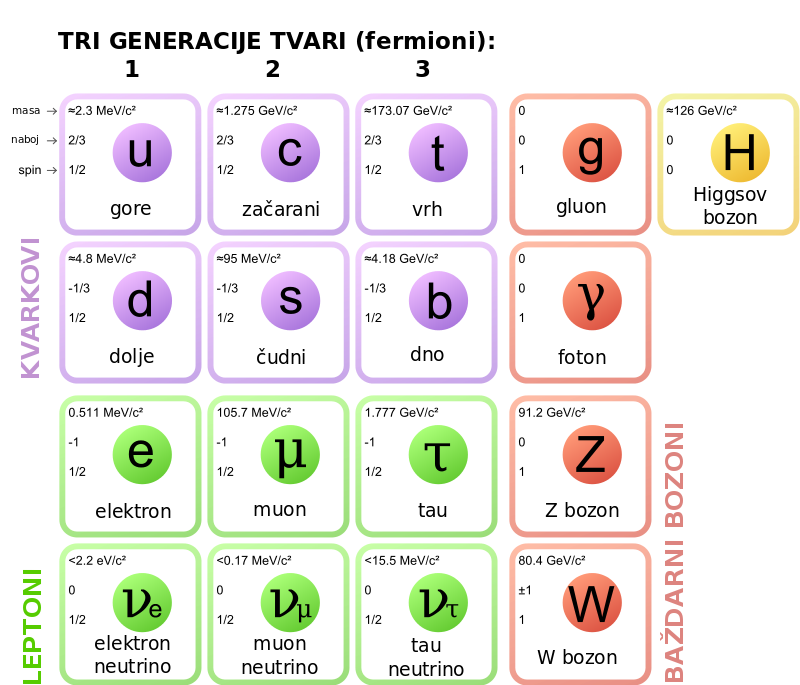
\includegraphics[width=0.8\textwidth]{Standard_Model_of_Elementary_Particles_hr.png}
			\caption[SM]{\label{sl:primjer}Tablica elementarnih čestica u standardnom modelu}
		\end{figure}
		
		
		\subsubsection{Fermioni}
		Fermioni su čestice spina 1/2 koje izgrađuju materiju i može ih se podijeliti u dvije podskupine: kvarkove i leptone, a svaka od podskupina  može se podijeliti u tri generacije. Svaki element veće generacije ima i veću masu s izuzetkom neutrina čija masa još nije točno izmjerena.
		\paragraph{Kvarkovi\newline}
		
		Do otkrića kvarkova, fizičari su znali samo za električni naboj koji je cjelobrojni višekratnik elementarnog naboja te se smatralo da je kvant elementarnog naboja jednak naboju elektrona, no sada vjerujemo da je kvant  jednak naboju kvarka. Ipak zbog povijesnih razloga ostali smo pri staroj notaciji pa tako elektron ima električni naboj -e, proton +e, jezgra helija +2e i tako dalje. Kvarkovi, ovisno o vrsti, imaju samo dio elementarnog naboj: +2/3e ili -1/3e. No, budući da kvarkovi ne postoje samostalno, već dolaze uvijek u kombinaciji dva ili tri kvarka, u prirodi nikad nije zapaženo postojanje čestice s nabojem manjim od jednog elementarnog naboja. Čestice sastavljene od 3 kvarka nazivamo barionima, dok mezonima nazivamo čestice sastavljene od para kvarka i antikvarka.Sva tvar (materija) u svemiru sastoji se od atoma, dakle od protona i neutrona, stoga su gornji i donji kvarkovi najviše zastupljeni kvarkovi u svemiru. Ostali kvarkovi su puno masivniji (masa kvarkova raste kako idemo od prve prema drugoj i trećoj generaciji) i puno rjeđi. Međutim, ranije u evoluciji svemira tvar je bila daleko energičnija, stoga su masivniji kvarkovi bili mnogo češći i imali su značajnu ulogu u reakcijama koje su se dogodile.
		
		\paragraph{Leptoni\newline}
		Od leptona najpoznatiji je elektron, stoga su leptoni najviše i proučavani budući da se svojstva elektrona zrcale u mionu i tau leptonu. Ova tri leptona imaju isti električni naboj i malo toga, osim mase, razlikuje elektron od miona i tau leptona. Jedina očita razlika je u tome što se mion i tau lepton mogu raspadati na druge čestice (iz prve i druge generacije leptona i njihove antičestice), dok je elektron stabilna čestica.Isto kao i kod kvarkova, masa leptona se povećava kako idemo prema višoj generaciji.
		Ostala 3 leptona se nazivaju neutrini jer su električki neutralni.
		Leptoni, za razliku od kvarkova, postoje u prirodi kao zasebne čestice. 
		Leptoni druge generacije su rjeđi, ali ih se može naći u prirodi. Mione je lako proizvesti u laboratorijskim pokusima. Osim po masi, vrlo su slični elektronima. Zbog velike mase su nestabilni pa se raspadaju na elektrone i neutrina. Članovi treće generacije nisu viđeni u nikakvim prirodnim procesima, barem ne u ovom stadiju evolucije svemira. Mnogo ranije, kada je svemir bio topliji i kada su čestice imale daleko više energije, leptoni treće generacije su često nastajali u prirodnim reakcijama. Danas se tau lepton može promatrati samo u laboratorijskim pokusima, dok tau neutrino nije izravno viđen u pokusima već se njegovo prisustvo daje zaključiti iz određenih reakcija.
		
		\subsubsection{Bozoni}
		Za razliku od fermiona koji izgrađuju materiju, bozoni su čestice međudjelovanja i njihov spin je cjelobrojan. Skupini baždarnih bozona, spina 1,  pripadaju fotoni,gluoni, W-bozoni i Z-bozoni, dok Higgsov bozon spada u skalarne bozone i njegov spin je 0.
		
		\paragraph{Fotoni\newline}
		Foton je osnovni djelić energije elektromagnetskog zračenja i on je elementarna čestica koja je posrednik u prenošenju elektromagnetskog međudjelovanja. U vakuumu se foton giba brzinom svjetlosti, a nema masu, električni naboj, ni energiju mirovanja.
		\paragraph{W i Z bozoni\newline}
		W i Z bozoni su elementarne čestice prijenosnici slabe nuklearne sile, odgovorne za raspade protona u neutrone i obrnuto. Za razliku od ostalih baždarnih bozona, mase mirovanja su im različite od nule, a iznose 80,4 i 91,2 GeV/c2, što je gotovo 100 puta više od mase protona, zbog čega im je djelovanje ograničeno na atomsku jezgru.
		\paragraph{Gluoni\newline}
		Gluon  je elementarna čestica bez mase, koja prenosi jako međudjelovanje i veže kvarkove u hadrone. Međudjelovanje kvarkova prenosi se emisijom i apsorpcijom gluona, slično kao što se elektromagnetsko međudjelovanje prenosi fotonima. 
		
		
		Valja naglasiti da i svaka čestica ima svoju antičesticu suprotnog kvantnog broja i najčešće joj simbol isti kao čestica samo s povlakom.
		
		
		\subsection{Lagrangian SM-a}
		SM teoretski možemo opisati objedinjenjem dvije teorije: kvantna elektrodinamika (eng. Quantum Electrodynamics QED) i kvantna kromodinamika (eng. Quantum Chromodynamics QCD). Sva tri međudjelovanja koja opisuje SM funkcioniraju u posredstvu nekog baždarnog bozona. Lagrangian SM-a je simetričan s obzirom na baždarnu grupu: 
		\begin{equation}
		SU(3)_C \times SU(2)_L \times U(1)_Y
		\end{equation}
		QCD teorija opisuje jako međudjelovanje i bazirana je na \begin{math}
		SU(3)
		\end{math}  grupi, dok  QED objašnjava elektroslabo međudjelovanje i simetrična je \begin{math}
		SU(2)_L \times U(1)_Y
		\end{math} grupi. ~\cite{doktorat}
		
		\subsubsection{Baždarna invarijantnost}
		Neka su električno i magnetsko polje opisani preko vektorskih i skalarnih potencijala na idući način:
		\begin{equation}
		\boldsymbol{E} = -\nabla \phi - \frac{\partial \boldsymbol{A}}{\partial t}
		\end{equation}
		\begin{equation}
		\boldsymbol{B} = \nabla \times \boldsymbol{A}
		\end{equation}
		Ako za potencijale vrijede baždarne transformacije:
		\begin{equation}
		\phi \rightarrow \phi + \frac{\partial \psi}{\partial t}
		\end{equation}
		\begin{equation}
		\boldsymbol{A} \rightarrow \boldsymbol{A} - \nabla \psi 
		\end{equation}
		to znači da električno i magnetsko polje nisu jedinstveno opisani, no baždarne transformacije su ih očuvale. Ako zapisujemo preko četverovektora potencijala i operatora diferencijala ,baždarna transformacija se može zapisati kao:
		\begin{equation}
		A_\mu \rightarrow A_\mu ^{'} = A_\mu + \frac{1}{e} \partial_\mu \alpha
		\end{equation}
		gdje e označava električni naboj.
		
		\paragraph{Lagrangian elektromagnetskog međudjelovanja\newline} 
		Ako Maxwellovu jednadžbu za slobodno elektromagnetsko (EM) polje  zapišemo u Lorentz kovarijantnom obliku:
		\begin{equation}
		\partial_\mu F_{\mu v} = 0
		\end{equation}
		gdje je \begin{math}
		F_{\mu v} = \partial_\mu A_v - \partial_v A_\mu 
		\end{math}
		tenzor jakosti EM polja, tada primjenjujući baždarne transformacije vidimo da tenzor ostaje ne promijenjen, stoga zaključujemo da je baždarno invarijantan što znači da su Maxwellove jednadžbe baždarno invarijantne.~\cite{dokt2} 
		Uvedimo sada Langrangian za slobodno elektromagnetsko polje:
		\begin{equation}
		L_{EM} = - \frac{1}{4} F_{\mu v} F_{v \mu}
		\end{equation}
		Baždarne tranfsormacije na tom Langrangianu se mogu opisati Abelovom grupom \begin{math}
		U(1)
		\end{math} . Kada govorimo o Abelovoj grupi mislimo na  matematički objekt linearne algebre čiji elementi zadovoljavaju svojstva: zatvorenosti, asocijativnosti, postojanje neutralnog elementa, postojanje inverznog elementa i komutativnosti.
		Ta grupa simetrije \begin{math}
		U(1)
		\end{math} ima jedan generator i to predstavlja postojanje jedne čestice medijatora elektromagnetne sile (fotona).~\cite{dokt2}
		Ukupni baždarno invarijantni Langrangian za QED je dan kao: 
		\begin{equation}\
		L_{QED}= -\frac{1}{4} F_{\mu v} F_{v \mu} + \bar{\psi}x [i \gamma^\mu (\partial_\mu - i e A_\mu) -m]\psi(x)
		\end{equation}
		\paragraph{Lagrangian elektroslabog međudjelovanja\newline}
		
		Isti princip baždarne invarijantnosti koji vrijedi za QED može se primijeniti na elektroslabo međudjelovanje koje zapravo objedinjuje dvije teorije međudjelovanja elektromagnetsko i slabo nuklearno. Ono obuhvaća  \begin{math}
		U(1)
		\end{math} grupu koja opisuje EM međudjelovanja i \begin{math}
		SU(2)_L
		\end{math} grupu koja opisuje ispospin slabog međudjelovanja. Grupa simetrije \begin{math}
		SU(2)_L \times U(1) 
		\end{math} ima 4 generatora što zapravo predstavlja 4 čestice medijatora, 3 za slabo međudjelovanje (\begin{math}
		W^+
		\end{math}, \begin{math}
		W^-
		\end{math} i \begin{math}
		Z
		\end{math} bozon), te 1 čestica za elektromagnetsko međudjelovanje(foton).
		
		Lagrangian elekroslabog međudjelovanja možemo zapisati kao:
		\begin{equation}\label{eq:3}
		\begin{split}
		L_{EW} = \bar{L}i\gamma^{\mu}\partial_\mu L + \bar{\psi '}_R i\gamma^{\mu}\partial_\mu \bar{\psi '}_R \\ - g_w \bar{L}\gamma^\mu \frac{\sigma_i}{2} L {W_\mu}^i - g \bar{L}\gamma^\mu \frac{Y}{2} L B_\mu - g \bar{{\psi'}_R}\gamma^\mu \frac{\sigma_i}{2} {\psi'}_R {B_\mu} \\ - \frac{1}{4}{W^{\mu v}}_i {W^i}_{\mu v} - \frac{1}{4}{B^{\mu v}} {B}_{\mu v}
		\end{split}
		\end{equation}
		~\cite{doktorat}
		
		\paragraph{Lagrangian jakog međudjelovanja\newline}
		Na sličan način kao i za elektroslabo međudjelovanje, grupa simetrije \begin{math}
		SU(3) 
		\end{math} ima 8 generatora tj. 8 čestica međudjelovanja u jakoj sili(gluoni). Langrangian takvog međudjelovanja dan je sa:
		\begin{equation}\label{eq:2}
		\begin{split}
		L_{QCD} = \bar{\psi_i}(i{(\gamma^\mu D_\mu)}_{ij} - m\delta_{ij})\psi_j - \frac{1}{4} G^a_{\mu v}G^{\mu v}_a 
		\end{split}
		\end{equation}
		
		
		
		\subsubsection{Spontano kršenje simetrije}
		Problem koji smo naveli u prošlom odlomku je vrlo elegantno riješen s tzv. BEH(Brout-Englert-Higgs) mehanizmom. To je zapravo mehanizam koji W i Z bozonima daje masu kada međudjeluju s nevidljivim poljem kojeg sada nazivamo Higgsovo polje. 
		Odmah nakon velikog praska iznos Higgsovog polje je bilo 0 ,no kako se svemir hladio i temperatura pala ispod kritične vrijednosti, polje je spontano raslo i kao posljedica toga u međudjelovanju s česticama davalo im masu. Kada se to ne bi događalo, ne bi ni bilo moguće razlučiti između 3 generacije elementarnih čestica jer po svim ostalim svojstvima su jednaki osim po masi. Što više čestica međudjeluje s poljem to teža postaje. Čestice poput fotona ne međudjeluju s poljem stoga ni nemaju masu. ~\cite{cernweb}
		Sam koncept Higgsovog mehanizma je veoma sličan efektu feromagnetizma u kojem zbog jakog međudjelovanja magnetskih momenata atoma dolazi do kolektivnog magnetskog uređenja tzv. spontane magnetizacije. U  vanjskom magnetskom polju, feromagnetične tvari postaju inducirani magneti koje zatim to polje privlači.  
		Naravno intuitivno je jasno i da za Higgsovo polje postoji čestica Higgsov bozon koji možemo zamisliti kao nekakvu pobudu u polju, kao npr. val na površini mora. ~\cite{cernweb}
		
		\paragraph{Lagrangian Higgsovog polja\newline}
		Očigledno je kako i za Higgsovo polje postoji Lagrangian~\cite{doktorat}:
		\begin{equation}\label{eq:4}
		\begin{split}
		L_{Higgs} = \frac{1}{2} \partial_\mu h \partial^\mu h + \mu^2 h^2 \\ + \frac{g_w^2 v^2}{4} {W^-}_\mu {W^{+\mu}} + \frac{g^2_w v^2}{8 \cos^2 \theta_w} Z_\mu Z^\mu \\ + \frac{g^2_w v^2}{2} h {W^-}_\mu {W^{+\mu}} + \frac{g^2_w }{4} h^2 {W^-}_\mu {W^{+\mu}} + \frac{g^2_w v}{4 \cos^2 \theta_w} h {Z}_\mu {Z^{\mu}} + + \frac{g^2_w}{8 \cos^2 \theta_w} h^2 {Z}_\mu {Z^{\mu}} \\ \frac{\mu^2}{v} h^3 + \frac{\mu^2}{4v^2} h^4
		\end{split}
		\end{equation}
		Važno je naglasiti da je masa Higgsovog bozona (\begin{math}
		m_H = \sqrt{|\mu|}
		\end{math})  slobodan parametar koji se ne može odrediti direktno iz teorije, već se mora izmjeriti.
		Također BEH mehanizam se iskoristio i za proširenje SM-a s baždarno invarijantnim Yukavinim članom koji je zadužen za davanje mase fermionima. On je zadan kao:
		\begin{equation}\label{eq:5}
			L_{Yukawa} = \sum_{f} -m_f \bar{\psi} \psi (1 + \frac{h}{v}) + \sum_{f'} -m_f \bar{\psi'} \psi' (1 + \frac{h}{v})
		\end{equation} 
		gdje prva suma ide po gornjem tipu fermiona, a druga po donjem tipu fermiona.
		
		Konačni Lagrangian SM-a možemo pisati kao sumu jednadžbi \ref{eq:2}, \ref{eq:3}, \ref{eq:4} i \ref{eq:5} 
		\begin{equation}
			L_{SM} = L_{QCD} + L_{EW} + L_{Higgs} + L_{Yukawa}
		\end{equation}
		~\cite{doktorat}
		
		\subsection{Higgsov bozon}
		Teoretski model koji smo opisali u prošlom poglavlju  je predložen još 70-ih godina prošlog stoljeća, no eksperimentalno je dokazan tek 2012. godine. 4. srpnja te godine CMS i ATLAS eksperiment su  objavili nepobitne dokaze o posljednjem velikom koraku koji je upotpunio SM kojeg poznajemo i dan danas. Nakon izbacivanja prvih  rezultata, znanstvenici iz europske organizacije za nuklearna istraživanja (fra. Conseil Européen pour la Recherche Nucléaire, CERN)  nastavili su nadograđivati Veliki Hadronski Sudarač (eng. Large hadron colider, LHC) te su dobivali sve pouzdanije i točnije rezultate. Najbolji primjer koliko se eksperiment razvio prikazuje slika \ref{sl:luminozitet}  koja pokazuje  porast luminoziteta  tijekom godina istraživanja, odnosno koliko se sudara dogodi u akceleratoru.~\cite{doktorat}
		
			\begin{figure}[h!]
			\centering
			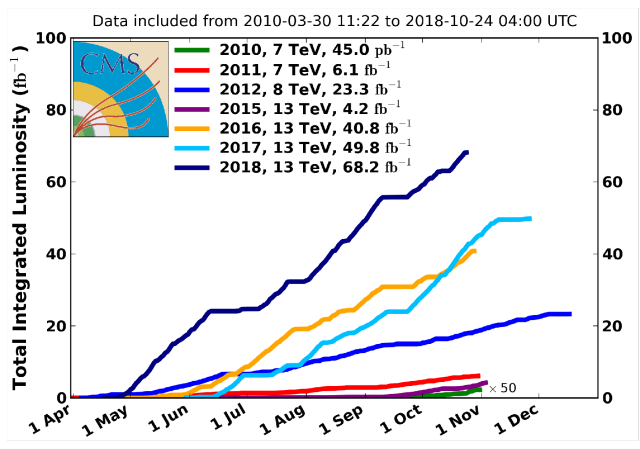
\includegraphics[width=0.8\textwidth]{luminozitet.png}
			\caption[Saturn viđen u ultraljubičastom svjetlu.]{\label{sl:luminozitet}Luminozitet u ovisnosti o godinama. }
		\end{figure}
		\subsubsection{Mehanizam produkcije Higgsovog bozona}
		Govoreći o SM-u neizbježno je spomenuti i Feynmanove dijagrame. To su grafičke ilustracije matematičkih izraza koje opisuju ponašanje i međudjelovanje subatomskih čestica, a uveo ih je američki fizičar Richard Feynman 50-ih godina 20. stoljeća. Oni će nam pomoći pri opisu glavnih mehanizama produkcije tj. nastajanja Higgsovog bozona. Iako postoji više načina za nastajanje Higgsova bozona mi ćemo se koncentrirati samo na one koji su mogući u LHC-u.~\cite{doktorat}
		
		\paragraph{Gluon fuzija\newline}
		Gluon fuzija je proces u kojem se dva gluona udružuju u međukoraknu petlju kvarkova, a potom iz te petlje nastaje Higgsov bozon. Taj proces je najčešći, što je pokazano najvećim udarnim presjekom od svih ostalih načina produkcije. Razlog tome leži u činjenici da je luminozitet gluona jako velik u proton-proton sudarima visoke energije koje LHC može proizvesti.
		\begin{figure}[h!]
			\centering
			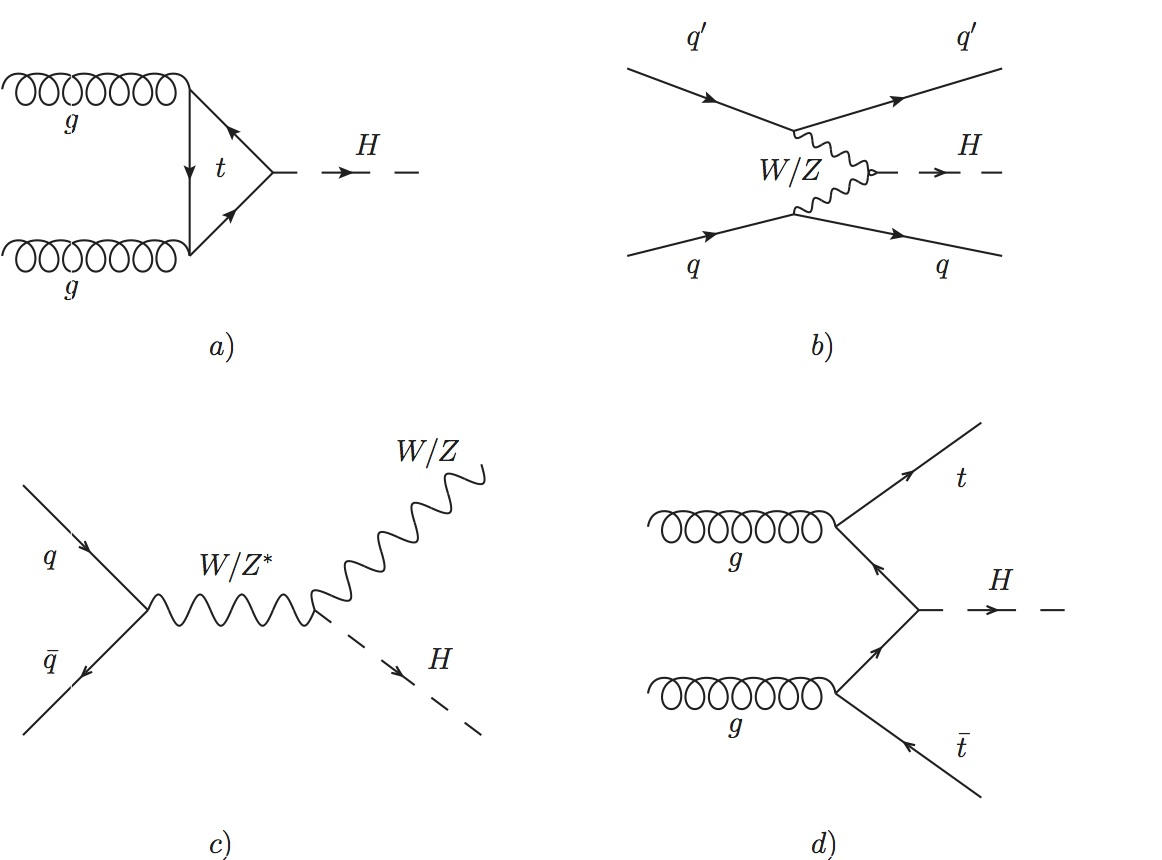
\includegraphics[width=0.8\textwidth]{higgs-production.jpg}
			\caption[Saturn viđen u  svjetlu.]{\label{sl:gluon-fuzija}a) Gluon fuzija, b)Vektor bozon fuzija, c)Procesi s pridruženom proizvodnjom W ili Z bozona, d)Procesi s pridruženom produkcijom \begin{math}
				\boldmath{t \bar{t}}
				\end{math}  para  }
		\end{figure}
		
		\paragraph{Ostali načini proizvodnje\newline}
		Vektor boson fuzija je drugi najčešći način produkcije Higgsovog bozona, ali udarni presjek tog procesa je manji za čak jedan red veličine od gluon fuzije. Ovaj proces se događa kada dva fermiona izmjene virtualne W ili Z bozone koji se trenutno udružuju i prelaze u Higgsov bozon. Eksperimentalno gledajući ovaj proces je veoma bitan za znanstvenike jer iz njega se vrlo jasno mogu prepoznati popratni visoko energizirani jetovi s velikom invarijantnom masom.
	
		Procesi s pridruženom proizvodnjom W ili Z bozona su treći najučestaliji način produkcije Higgsovog bozona. U tom procesu se fermion i antifermion sudare i proizvedu W ili Z bozon koji nakon toga izrači Higgsov bozon. Kao izlaz u tom procesu vidimo Higgsov bozon koji je popraćen sa leptonskim ili hadronskim česticama koji su proizvod  W ili Z bozona.
		
		Procesi s pridruženom proizvodnjom \begin{math}
		\boldmath{t \bar{t}}
		\end{math}  para su najrjeđi od svih procesa. U ovom procesu dva gluona u sudaru se raspadaju u dva para kvarkova i anti kvarkova i tada kvark iz jednog para produkta i antikvark iz drugog para udružuju se u Higgsov bozon. Za posljedicu ovog procesa vidimo izračeni par preostalih kvark i antikvark čestica.
		
		\subsubsection{Mehanizmi raspada Higgsovog bozona}
		U teoriji kvantne fizike vrijedi pravilo "ako se čestica može raspasti na lakše čestice to će i učiniti". Higgsov bozon nije iznimka. Kao što se Higgsov bozon može proizvesti na više načina tako i postoje razne varijacije u njegovom raspadu. Za Higgsa mase \begin{math}
		125 Gev/c^2
		\end{math} SM predviđa se vrijeme života od otprilike \begin{math}
		1.6 * 10^-22
		\end{math} s. To znači da kad se Higgs proizvede u sudaru, dok dođe do detektora već će se raspasti i kao takvog ga ne možemo prepoznati. Iz tog razloga mi promatramo čestice i njihova svojstva koje nastaju u raspadu Higgsa. Na temelju tih svojstva određujemo karakteristike Higgsova bozona.
	
	Jedan od takvih načina raspada je i cijepanje Higgsa u fermion anti-fermion par. Generalno pravilo je da će se Higgs prvo raspasti na teže fermione pa tek onda na lakše, jer je masa fermiona proporcionalna jačini veze s Higgsom. Po toj logici najčešći raspad bi bio na gornji (eng. top) , anti-top kvark, no ipak za takav raspad potreban bi bila energija od \begin{math}
	346Gev/c^2
	\end{math}. Iz tog razloga Higgs mase \begin{math}
	125 Gev/c^2
	\end{math} se raspada na donji(eng. bottom) anti-bottom kvark par i to se događa u 57.7\% situacija. Drugi najčešći u kategoriji fermion-antifermion je raspad na tau lepton anti-tau lepton par i to se događa u 6.3\% slučajeva.
		
		Druga kategorija raspada Higgsa je u masivne baždarne bozone. U 21.5\% slučajeva raspada se u par W bozona, a onda se isti mogu raspast u kvark anti-kvark par ili pak u nabijen lepton i neutrino. Takav raspad W bozona je jako teško razlučiti od pozadine, a raspad u leptone je gotovo nemoguće rekonstruirati zbog slabe detekcije neutrina. 
		Ljepši raspad je pak raspad u parove Z bozona i to se događa samo u 2.6\% slučajeva, i par se poslije raspada u leptone koje je lako detektirati.
		
		Raspad na ne masene baždarne bozone(gluone i fotone) je također moguć,no takav raspad sadrži i međukoraknu petlju virtualnih kvarkova. U 8.6\% slučajeva dogodit će se raspad na gluone, dok najrjeđi od svih je raspad na fotone u samo 0.86\%. No unatoč tome što je jako rijedak, jako je značajan jer se količina gibanja i energija može mjeriti jako precizno što daje izrazito točne rezultate pri rekonstrukciji Higgsovog bozona.
		
		
		\subsection{Kanal raspada \begin{math}
			H \rightarrow ZZ* \rightarrow 4\mu \end{math}}
		Od svih navedenih tipova raspada u ovom diplomskom radu bavit ćemo se samo onim u kojem se Higgsov bozon raspada na par Z bozona, a potom i oni u 4 muona. . No ipak ako pronađemo 4 muona ne znači da smo pronašli Higgsov bozon odnosno da su oni nastali iz Higgsovog bozona. Razlog tome leži u činjenici da parovi Z bozona mogu nastati i iz drugih reakcija koje predviđa SM, poput fuzije gluona ili anihilacije kvark antikvark para.
		Unatoč tome što samo 0.0124\% svih sudara gdje se pojavi Higgs mase \begin{math}
		125 Gev/c^2
		\end{math} rezultira ovim kanalom raspada jedan je od najznačajnijih. Razlog tome je što možemo napraviti potpunu rekonstrukciju objekata finalnog stanja čak i za jako malo energije. Rezolucija momenata za elektrone i muone je jako dobro i stoga je moguće jako precizno mjeriti masu Higgsovog bozona i možda najvažnije, omjer signala i pozadine je odličan čak 2:1 što znači da i kad umanjimo pozadinu i pritom izbrišemo signale, ostat će nam dovoljno signala za zdravu analizu. Ovaj kanal nam je također jako koristan jer uz samu mjerenje mase Higgsova bozona, moguće je mjeriti i jačinu signala, spin-pariy, fiducial cross section, parove anomalaija ili pak tražiti masivnije Higgsove bozone.
		
		
		
		\section{LHC sudarivač i CMS eksperiment}
		\subsection{Povijest CERN-a}
		CERN organizacija  osnovana je 29. rujna 1954. godine od strane 12 zemalja Zapadne Europe. Izvorno, CERN je bio akronim za francuske riječi Conseil Européen pour la Recherche Nucléaire, no danas institut nosi naziv Organisation Européenne pour la Recherche Nucléaire. Ipak radi branda i povijesnih razloga zadržan je akronim CERN. Laboratorij je izvorno bio namijenjen istraživanju jezgre atoma, ali se ubrzo nakon toga prebacio na istraživanje međudjelovanja subatomskih čestica. Danas, CERN je najveći laboratorij za fiziku visokih energija na svijetu. Nalazi se na sjeverozapadnoj strani Ženeve na Francusko-Švicarskoj granici i sastavljena je od 23 članice država svijeta. 
		Glavna zadaća CERN-a je omogućavanje provođenja eksperimenata u fizici visokih energija s ubrzivačima čestica i ostalom infrastrukturom koja bi nezavisnim znanstvenicima bila jako skupa i teško dostupna.  Iako je u CERN-a izvedeno  mnogo uspješnih eksperimenata, ovo su glavna postignuća u bogatoj povijesti njegova rada ~\cite{cern-wiki}:
		\begin{itemize}
		\item 1973. Otkriće neutralnih struja
		\item 1983. Otkriće W i Z bozona
		\item 1989. Utvrđivanje broja neutrinskih vrsta
		\item 1995. Prvo stvaranje atoma antivodika
		\item 1999. Otkriće izravnog CP-narušenja
		\item 2010. Izolacija 38 atoma antivodika
		\item 2011. Održavanje antivodika više od 15 minuta
		\item 2012.Otkriće Higgsovog bozona 
		\end{itemize}
		
		\subsection{LHC}
		LHC je najveći i najmoćniji ubrzivač čestica na svijetu. Pušten je u pogon 10.rujna 2008. godine kada je zamijenio dotadašnje sustave Protonskog Sinkotrona (eng. Proton Synchrotron, PS) i Super Protonskog Sinkotrona (eng. Super Proton Synchrotron, SPS) prikazane na \ref{sl:schema-lhc}.
		
		\begin{figure}[h!]
			\centering
			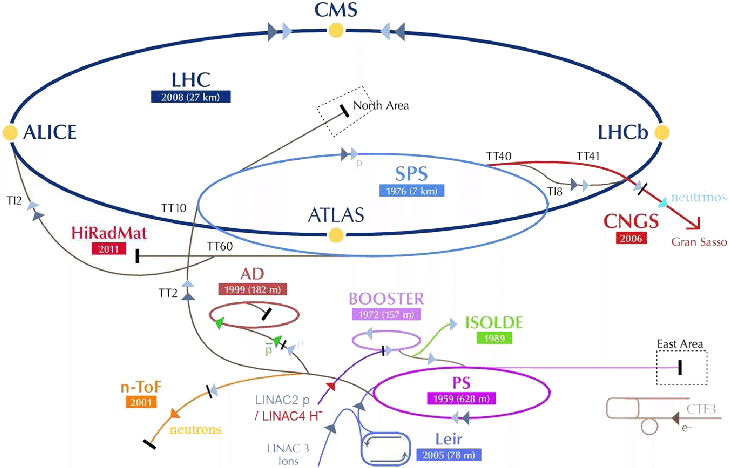
\includegraphics[width=0.8\textwidth]{schema-lhc.png}
			\caption[Saturn viđen u ultraljubičastom svjetlu.]{\label{sl:schema-lhc}Schema LHC-a u CERN-u }
		\end{figure}
		Unutar samog ubrzivača, prije nego se sudare, putuju dvije visoko energizirane zrake čestica koje se gibaju brzinom bliskoj brzini svjetlosti. Zrake putuju unutar dvije odvojene cijevi u suprotnim smjerovima, a same cijevi su pod visokim vakuumom. Zrake su dovedene do brzine svjetlosti sa snažnim magnetskim poljem supravodljivih elektromagneta, koji su izgrađeni od zavojnica specijalnog materijala koji se ohladi na -271.3 \degree C te omogućuje bez otporni tok struje, tj. omogućuje da se ne gubi nikakva energija. Iz tog razloga, cijeli akcelerator je umrežen u sistem tekućeg helija. Tisuće magneta raznih oblika i veličina usmjeruje zrake kako bi točno prije sudara zraka bile na istoj poziciji s većom vjerojatnošću udarnog presjeka. Radi dobivanja osjećaja možemo reći da je taj sustav toliko precizan kao da ispalimo dvije igle na 10 km udaljenosti i želimo da se sudare.
		Sami sudari se događaju u 4 različita detektora ATLAS, CMS, ALICE i LHCb.~\cite{cern-lhc}
		
		\subsection{CMS}
		Kompaktni muonski solenoid (eng. Compact Muon Solenoid, CMS) jedan je od 4 detektora koja postoje u LHC-u i ovo su njegove glavne karakteristike:
		\begin{itemize}
			\item kompaktnost – relativno je malen s obzirom na svoju masu
			\item muonski – napredni sustav za detekciju muona
			\item solenoid – supravodljivi solenoid
		\end{itemize}
	
		Kako je masa Higgsovog bozona slobodan parametar u SM-u, moralo je se tražiti u širokom energetskom rasponu od 100 GeV do 1 TeV. To je značilo da je detektor morao biti sposoban rekonstruirati i identificirati objekte u finalnom stanju nakon raspada iz Higgsovog bozona. Također detektor je morao biti dovoljno brz da analizira sve bitne događaje u sudarima, ali isto tako da preživi visoku radijaciju koja se događa u istim.
		Detektor se nalazi 100 m ispod malog francuskog sela Cessy. 21 metara dug,15 metara širok te 15 metara visok, CMS je kao veliki filter sa strukturom luka. Svaki sloj je zadužen za mjerenje i zaustavljanje različite vrste čestica. Detektor je izgrađen oko velikog magnetnog solenoida u obliku cilindra koji je ohlađen na -268.5 \degree C i generira polje od 4 T, što je oko 100 puta jače od magnetskog polja Zemaljske kugle.
		Čestice nastale u sudaru  \ref{sl1:cms-scheme} prvo prolaze kroz tracker sistem koji detektira putanju elektrona. Cijeli tracker se nalazi pod jakim magnetskim poljem od 4T kojim se može vrlo precizno zakriviti elektron i izvući njegova svojstva poput količine gibanja. Izvan trackera nalazi se elektromagnetski kalorimetar (eng. Electromagnetic Calorimeter, ECAL) koji namjenjen za detekciju i zaustavljanje fotona i elektrona. Idući sloj je hadronski kalorimetar (eng. Hadronic Calorimener, HCAL) zadužen za detekciju i zaustavljanje hadrona i nešto je salbijeg magnetskog polja od otprilike 3.8T. Sve to obavijeno je supravodljivim solenoidom zaduženim za generiranje tako snažnih magnetskih polja. Konačno, 4 sloja muonskih detekrora i željeznih barijera služe za detekciju i zaustavljanje muona pod magnetskim poljem od 2T.
		\begin{figure}[h!]
			\centering
			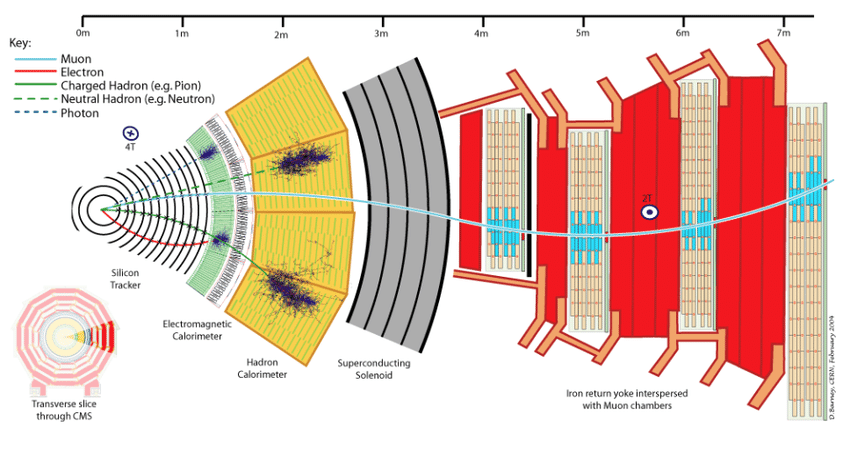
\includegraphics[width=0.8\textwidth]{cms-scheme.png}
			\caption[Saturn viđen u ultraljubičastom svjetlu.]{\label{sl1:cms-scheme}Schema CMS detektora u CERN-u }
		\end{figure}
	
		\subsubsection{Sistem okidača}
		Pri maksimalnom opterećenju u CMS-u se sudari događaju svakih 25ns i nije moguće zabilježiti svaki od sudara. Zato je razvijen sustav okidača da bi zabilježili samo one događaje visokih energija  koji su nam posebno važni. Sustav je sastavljen od 3 koraka, gdje je L1 kompletno hardverski, dok su L2 i L3 softverski i objedinjeni su u visoko razinski okidač (eng. High level trigger, HLT).
		L1 razinski okidač spusti frekvenciju sudara koje prihvaćamo sa 40MHz na samo 100kHz. Kako ne bi miješao čestice iz dva različita sudara dozvoljen je odmak od samo 4 {$\mu$}s. Ako je uvjet zadovoljen šalje se na obradu u HLT sustav, a ako ne sudar se odbacuje. Zbog hardverske ograničenosti L1 sustav funkcionira samo na kalorimetrima i muonskim komorama
		Ako prođe L1 sustav okidača, sudar dolazi na softversku obradu koja zahtjeva ispunjavanje raznih uvjeta kao npr. postojanje dva izolirana elektrona.  U konačnici finalni ispis je samo 1kHz frekvencije.~\cite{doktorat}
		
		\subsubsection{Rekonstrukcija čestica}
		Kao što smo već naveli, neke čestice imaju kratki vijek života i nemoguće ih je direktno detektirati. Iz tog razloga potrebno je napraviti rekonstrukciju čestica nastalih u procesu raspada naše željene čestice. Svaka čestica koja se detektira može nastati iz više elemenata i glavni cilj kod rekonstrukcije je povezati različite čestice u različitim detektorima s istom izvornom česticom. 
		Rekonstrukcija se može razbiti u 3 grube kategorije: praćenje tragova, algoritam klastera i algoritma čestičnog toka (eng. Particle-flow, PL).
		Praćenje tragova se odvija tako da se promatra trag čestice koja prolazi kroz magnetsko polje. Znajući snagu tog magnetskog polja možemo znati i svojstva dane čestice. Tracker može rekonstruirati putanje visoko-energiziranih muona, elektrona i hadrona. Također od trackera se očekuje da bude dovoljno precizan do na 10 $\mu$m, ali opet toliko nježan da ne utječe na samu česticu ~\cite{cern-tracker}.
		Svrha algoritma klastera u kalorimetru je detektiranje i mjerenje energije  i putanje stabilne neutralne čestice, odvajanje neutralnih čestica od nabijenih hadronskih deposita energije, te rekonstrukcija i identifikacija elektrona  s popratnim zakočnim zračenjem fotona.
		PF algoritam objedinjuje cijelu rekonstrukciju u jednu cijelinu, no radi kompleksnosti ovog algoritma mi ćemo u ovom diplomskom opisati samo praćenje tragova muona i njihovu rekonstrukciju.
		
		S PF algoritmom možemo rekonstruirati 3 različita tipa muonskih kandidata:
		\begin{itemize}
			\item Muoni koji stoje sami za sebe
			\item Globalni muoni
			\item Muoni tragova 
		\end{itemize}
		Čak 99\% rekonstruiranih muona su globalni ili muoni tragova. Globalni muoni popravljaju rezoluciju momenata, a muoni tragova popravljaju učinkovitost muona s niskom količinom gibanja koji ne uspiju u potpunosti prijeći cijeli CMS detektor. Globalni muoni i muoni tragova koji imaju isti trag se povezuju u jednog kandidata. Muoni koji stoje sami za sebe inače imaju lošiju rezoluciju momenata i veću mješavinu kozmičkih miona nego globalni i muoni tragova.
		Naboj i količina gibanja PF muona se uzima iz fita tragova ako je količina gibanja manja od 200 GeV. Iznad te vrijednosti količina gibanja se uzima prema najmanjoj chi-square vjerojatnosti iz fita za različite tragove. Naravno da pri ovakvoj rekonstrukciju može doći do pogreške i druge čestice se rekonstruira kao muone i onda oni predstavljaju pozadinu.~\cite{doktorat}
		
		\newpage
		\section{Analiza kanala raspada \begin{math}
		\boldmath	{H \rightarrow ZZ^* \rightarrow 4\mu }\end{math} }
		Kako bi što bolje opisali svojstva Higgsovog bozona u SM-u jako je bitno da odredimo koje ćemo događaje promatrati proizvedene u CMS detektoru.
		Proces odabira događaja u ovoj analizi fokusira se na dobivanje što više signala Higgsovog bozona sa što manje pozadine. Također veoma bitan korak ove analize je odabir opservabli kojima možemo odijeliti signal i pozadinu. Govoreći o pozadini postoje dvije vrste: reducibilna i ireducibilna pozadina. 
		Ireducibilna pozadina ima isto finalno stanje kao i signal, no nastala je iz drugog procesa SM-a. Npr. Za naš kanal \begin{math}
		H \rightarrow ZZ^* \rightarrow 4\mu \end{math}, procesi ireducibilne pozadine bi bili \begin{math}
		gg \rightarrow ZZ
		\end{math} i \begin{math}
		qq \rightarrow ZZ
		\end{math} te bi se Z bozoni raspadali na 4 muona. Za razliku od ovakvih procesa koje nije teško simulirat, problem stvaraju procesi s reducibilnom pozadinom. To su procesi u kojem su finalni objekti krivo protumačeni u detektoru kao muoni nastali iz Z bozona. Dominantni izvori takvih događaja su Z bozoni i jetovi, gdje npr. Heavy flavour jetovi proizvode sekundarne leptone ili gdje se raspadanje nabijenih hadrona preklapa s raspadom piona i onda tumačimo to kao leptone. 
		Važno je promatrati sve moguće raspade,a onda sve objediniti statističkom analizom u kojoj preko likelihooda mjerimo neki parametar od interesa poput mase Higgsovog bozona.~\cite{doktorat}	
	
		\subsection{Podaci i Montecarlo simulacije}
		Važnost teoretskog modela SM-a opisanog u drugom poglavlju ovog rada tek sada dolazi do izražaja.  Taj model je krucijalni korak u eksperimentalnim mjerenjima Higgsovog bozona u CMS-u. Kako smo već prethodno naglasili, teoretski model ne daje pravu vrijednost mase Higgsovog bozona već je moramo mjeriti. Isto tako vrijeme života Higgsovog bozona je prekratko da bi se direktno detektirao kao čestica već detektiramo čestice finalnog stanja koje su nastale pri raspadu Higgsa. Sa SM-om možemo izračunati vjerojatnosti stvaranja i raspada Higgsa po različitim kanalima. To nam je vrlo važno kod stvaranja Montecarlo (MC) simulacija. MC simulacije su računalni algoritmi koji se temelje na uzorkovanju slučajnih brojeva kako bi opisali nekakav problem koji može biti determinističke prirode ~\cite{mc-simulacije}. U našem konkretnom slučaju, preko MC-a možemo simulirati kako se Higgs stvara i raspada s pripadajućim vjerojatnostima. Tako simulirani podaci nam mogu vrlo dobro opisati model kojim ćemo promatrati prave izmjerene podatke u detektoru.
		
		\paragraph{Težina događaja}
		Kada prvotno simuliramo podatke koji se stvaraju u detektoru svaki događaj ima istu važnost(pišemo 1), no takva simulacija ne bi bila dobra. Neki događaju su više, a neki manje vjerojatni. Zato je bitno da svakom događaju dodijelimo težinu(eng. Weight) koji predstavlja vjerojatnost zbivanja istog.
		Formula za izračunavanje težine događaja u ovom diplomskom radu je dana s:
		\begin{equation}
		težina\textunderscore događaja = \frac{lumi*1000*xsec*kfactor*overallEventWeight*L1prefiringWeight}{gen\textunderscore sum \textunderscore weight}
		\end{equation}
		gdje lumi predstavlja ukupni luminozitet i uzimamo ga kao 137/fb, xsec udarni presjek danog procesa, kfactor .... te ga uzimamo 1 za pozadinu, overallEventWeight ......, L1prefiringWeight......, gensumweights ...... , a ako se radi o signalu nastao gluon-gluon fuzijom još množimo sa ggHNNLOPSweight.
		
		\subsection{ROOT i RooFit}
		Radi kompleksnosti izrade MC simulacija, ja sam u ovom radu dobio već gotove simulirane podatke prema kojima mogu raditi model. Ti podaci su bili u obliku ".root" datoteka. Ekstenzija takve datoteke dolazi od ROOT , objektno orijentiranog programa te biblioteke razvijena u CERNU-u. Primarno je bila razvijena za analizu podataka u čestičnoj fizici, no danas se također koristi u astronomiji i rudarenju podataka~\cite{roofit}. Glavno obilježje ROOT datoteka je da se podaci pohranjuju u tzv. stablo(eng. Tree) koje ima svoje substrukture grane(eng. Branches) i listove(eng. Leaves).  Stablo je vrlo elegantan način za spremanje podataka jer izbjegava probleme kod alociranja memorije kod stvaranja objekata ,a samo spremanje se obavlja vrlo brzo. Uz samu root biblioteku koristio sam se ponajviše njenim proširenjem RooFit s kojim se na vrlo elegantan način rješavaju kompleksni problemi prilagodbe podataka na nekakav model. ROOT biblioteku sam implementirao s C++ koji je i dan danas jedan od najbržih računalnih programa na svijetu.
		
		\subsection{Statistička analiza}
		Kada smo dobili podatke koji simuliraju raspad Higgsovog bozona prema SM-u, idući korak je prilagodba (eng. Fit) tih podataka na nekakav model tj. funkciju koja najbolje opisuje njihovu raspodjelu.
		
		\subsubsection{Funkcija gustoće vjerojatnosti}
		Funkcija gustoće vjerojatnosti (eng. Probability density function, PDF) nam govori kolika je vjerojatnost da izmjerimo neku vrijednost x u rasponu \begin{math}[x-dx, x+dx]
		\end{math}. Općenito integral po cijelom rasponu te funkcije je uvijek 1, što u suštini znači da je vjerojatnost mjerenja vrijednosti po cijelom području 100\% odnosno da ćemo sigurno negdje pronaći našu traženu vrijednost.
		Vjerojatno najpoznatiji PDF je Gaussian. 
		\begin{figure}[h!]
			\centering
			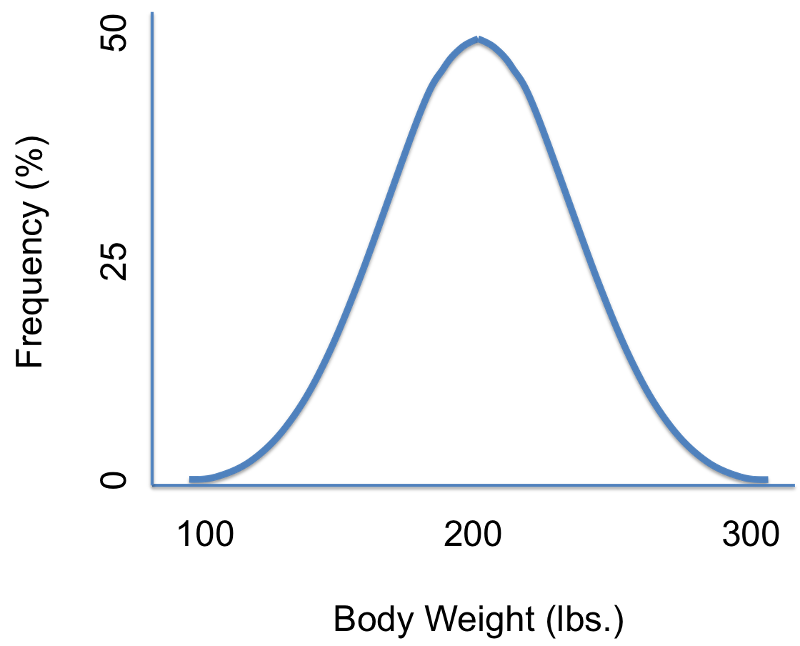
\includegraphics[width=0.8\textwidth]{gauus.png}
			\caption[Saturn viđen u ultraljubičastom svjetlu.]{\label{sl:gauss} Raspodjela po masi ljudi }
		\end{figure}
		Radi laičkog razumijevanja, Gaussovom krivuljom možemo npr. opisati tjelesnu masu kod ljudi. Ako slučajnim odabirom promotrimo masu neke odrasle osobe, najvjerojatnije da će njegova/njena tjelesna masa biti oko srednje tjelesne mase svih ljudi, a najmanje vjerojatno da će biti u ekstremnim granicama promatranog uzorka. Uz Gaussovu raspodjelu, koju zovemo još i normalna raspodjela, poznate su još i chi-square, eksponencijalna, gamma, Landau, crystall ball itd.
		
		\subsubsection{Likelihood funkcija}
		Ako pretpostavimo da su svi događaju međusobno nezavisni, onda je vjerojatnost za N događaja dan kao produkt vjerojatnosti svakih od pojedinačnih događaja:
		\begin{equation}
		P(x;\theta) = P(x_1 ; \theta) P(x_2 ; \theta) \cdot \cdot \cdot P(x_N ; \theta) = \prod P(x_i ; \theta)
		\end{equation}
		Kada se varijabla x zamjeni opservablom \begin{math}
		x^{OBS}
		\end{math} tada P nije više PDF, već likelihood funkcija  koja se označava sa \begin{math}
		L (x^{OBS}; \theta)
		\end{math}. Vjerojatnost odvijanja N nezavisnih događaja je dana s:
		\begin{equation}
		L(x; \theta) = \prod f(x_i; \theta)
		\end{equation}
		
		Maximum likelihood estimator \begin{math}
		\hat{\theta}
		\end{math} je vrijednost $\theta$ za koji je funkcija likelihooda postiže najveću vrijednost. Traženje maksimuma se može provesti na standardan način,deriviranjem funkcje L i izjednačavanjem s 0, no ipak je bolje tražiti maksimum log-likelihood funkcije:
		 \begin{equation}
		 ln L(x; \theta) = \sum ln f(x_i; \theta)
		 \end{equation}
		 jer je operacija množenja zamijenjena operacijom zbrajanja koja je računalno puno jednostavnija.
		 Ovdje valja naglasiti da procjena maksimumlikelihooda nije najvjerojatnija vrijednost traženog parametra, već je najbolja procjena naših uzorkovanih podataka.
		
		\subsubsection{Statističke i sistematske pogreške}
		........................................................
		
		
		Cijela statistička analiza opisana u ovom poglavlju je implementirana u pozadini RooFit programskog paketa, koji automatski radi fit na dane podatke.
		
		\newpage
		\section{Rezultati}
		\subsection{Signal i pozadina}
		Simulirani podaci koje sam dobio predstavljaju signal u kanalu proizvodnje gluon-gluon fuzije koji čini gotovo 90\% svih nastanaka Higgsovog bozona. Drugi najčešći način produkcije, vektor bozon fuzije, smo obradili na osnovnoj razini jer se zbiva u tek oko 9\% slučajeva. Kao što smo već naglasili u dosadašnjem tekstu, promatramo samo kanal raspada na 2 Z bozona,a potom na 4 muona. U našim podacima osim muonskih, sadržani su i ostali leptonski događaji, pa smo morali postaviti i uvjet odabiranja samo mion-antimion parova.
		Za pozadinu smo dobili dvije simulirane datoteke podataka, gg $\rightarrow$ ZZ$\rightarrow$ 4mu, te qq$\rightarrow$ ZZ$\rightarrow$ 4mu koje predstavljaju ireducibilnu pozadinu (//KAKAV JE LANDAU).
		
		Kao što smo već spomenuli, većina signala dolazi iz gluon-gluon fuzije pa je bilo intuitivno prvo započeti s prilagodbom podataka na funkciju upravo te vrste signala.
		Prvo sam pokušao podatke prilagoditi na Gaussovu krivulju \ref{sl:gauss-fit}, no uočeno je veliko neslaganje.
		\begin{figure}[h!]
			\centering
			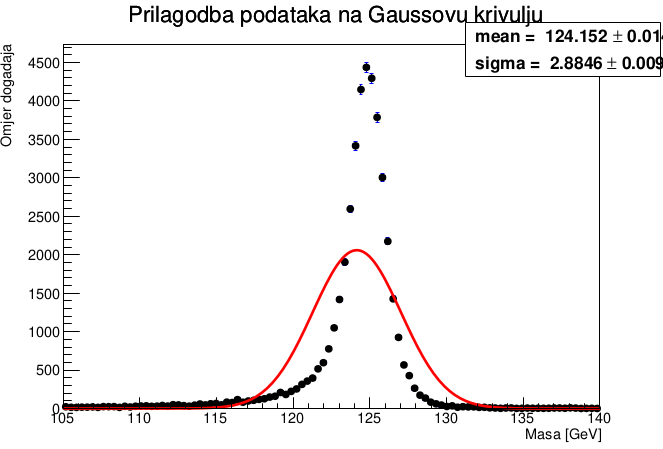
\includegraphics[width=0.8\textwidth]{gauss-fit1.png}
			\caption[Saturn viđen u ultraljubičastom svjetlu.]{\label{sl:gauss-fit} Prilagodba podataka na Gaussovu krivulju}
		\end{figure}
		Iz grafa je jasno vidljivo da tražimo neku funkciju koja ima manju širinu sigma oko srednje vrijednosti. Funkcija takvog oblika bi bila najbliža crystall ball koja je zadana kao:
		\begin{equation}
		\begin{split}
		f(x; \alpha, n, \bar{x}, \sigma)= N \cdot \begin{cases}
		exp(- \frac{(x-\bar{x})^2}{2\sigma^2}),& \frac{x-\bar{x}}{\sigma}> -\alpha\\
		A \cdot (B- \frac{x-\bar{x}}{\sigma})^{-n},& \frac{x-\bar{x}}{\sigma} \leqslant - \alpha
		\end{cases}\\
		A = (\frac{n}{|\alpha|})^n \cdot exp(- \frac{|\alpha|^2}{2}), \\
		B = \frac{n}{|\alpha|} - |\alpha|, \\
		N = \frac{1}{\sigma (C+D)}, \\
		C = \frac{n}{|\alpha|} \cdot \frac{1}{n-1} \cdot exp(- \frac{|\alpha|^2}{2}), \\
		D = \sqrt{\frac{\pi}{2}} (1+erf(\frac{|\alpha|}{\sqrt{2}}))
		\end{split}
		\end{equation}
		, gdje je N faktor normalizacije, $\alpha$, n, $\sigma$ i $\bar{x}$ parametri koji se prilagođavaju na podatke, a erf funkcija pogreške.
			\begin{figure}[h!]
			\centering
			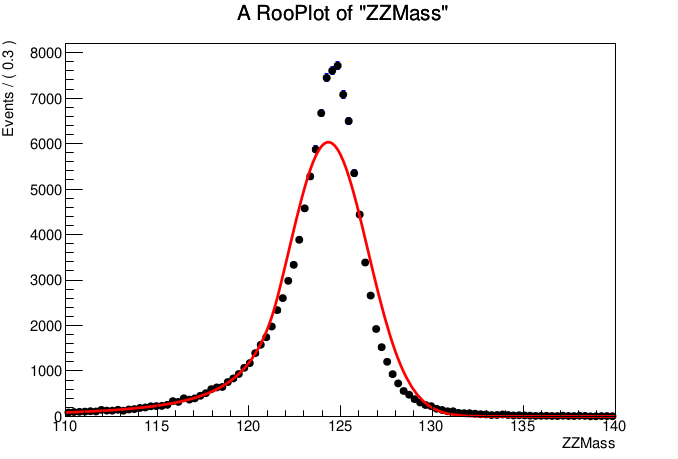
\includegraphics[width=0.8\textwidth]{cbfit.png}
			\caption[Saturn viđen u ultraljubičastom svjetlu.]{\label{sl:cbfit} Prilagodba podataka na Crystall ball krivulju}
		\end{figure}
		Iako krivulja puno bolje opisuje podatke i dalje ne uspijeva dosegnuti svoj peak.
		Idealna funkcija koja može ispuniti taj uvjet je double crystall ball, koja ima "rep" s obje strane za razliku od obične crystall ball koja ima rep samo s jedne strane.
		U konačnici dobivamo \ref{sl:dcbfit}
		\begin{figure}[h!]
			\centering
			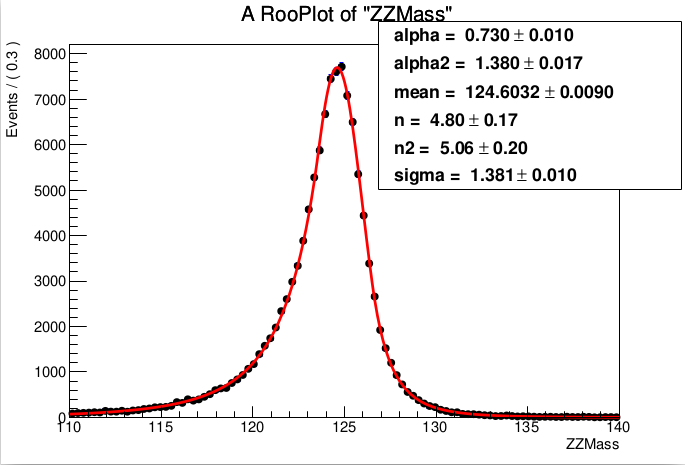
\includegraphics[width=0.8\textwidth]{dcbfit.png}
			\caption[Saturn viđen u ultraljubičastom svjetlu.]{\label{sl:dcbfit} Prilagodba podataka na Double Crystall ball krivulju}
		\end{figure}
	
		 Promatranjem golim okom funkcija izgleda savršeno, no parametarski treba uvesti još i težine događaja. Taj korak će ponajviše doći do izražaja kad napravimo ukupni model u kojem smo ukomponirali sve pozadine i signal, jer upravo suma svih težina pojedinačnih događaja predstavlja integral, tj. površinu ispod krivulje funkcije.
		  
		\begin{figure}[h!]
			\centering
			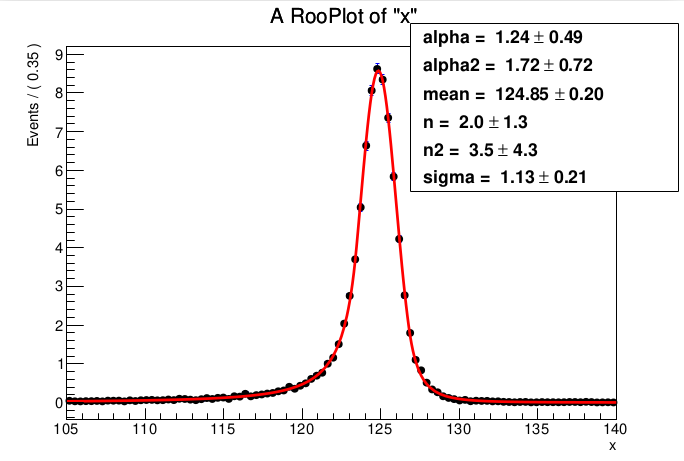
\includegraphics[width=0.8\textwidth]{dcbfit-weight.png}
			\caption[Saturn viđen u ultraljubičastom svjetlu.]{\label{sl:dcbfitweight} Prilagodba podataka na Double Crystall ball krivulju sa prilagođenim težinama podataka}
		\end{figure}
	
		Kako bi se uvjerili u točnost modela također smo napravili i maximum likelihood za pojedine parametre, no ipak srednja vrijednost nam je bila najzanimljivija.
		
		\begin{figure}[h!]
			\centering
			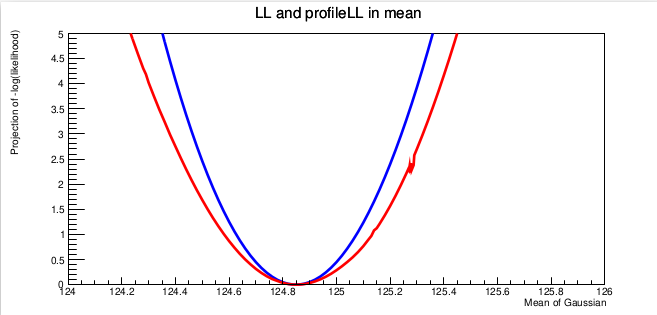
\includegraphics[width=0.8\textwidth]{maxlike-mean.png}
			\caption[Saturn viđen u ultraljubičastom svjetlu.]{\label{sl:maxlike-mean} Maximum likelihood i profile likelihood za srednju vrijednost u signalnom modelu}
		\end{figure}
	
		Istu proceduru ponovimo i za pozadine. 
		Za pozadinu ZZ $\rightarrow$ 4mu podatke smo opisali polinomom drugog reda\ref{sl:background-zz}, dok smo gg $\rightarrow$ 4mu običnom linearnom funkcijom \ref{sl:background-gg}. Naravno bilo je za očekivati velike pogreške prilikom fita parametara, no unatoč tome funkcija jako dobro opisuje naše podatke. Razlog velikim pogreškama su isto tako velike oscilacije (......zašto točno.....)
		
		\begin{figure}[h!]
			\centering
			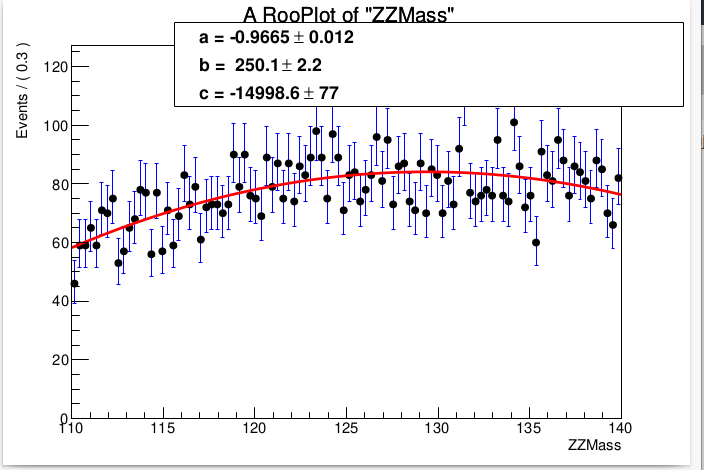
\includegraphics[width=0.8\textwidth]{background-zz.png}
			\caption[Saturn viđen u ultraljubičastom svjetlu.]{\label{sl:background-zz} Prilagodba pozadine ZZ $\rightarrow$ 4mu na polinom II.stupnja}
		\end{figure}
	
		\begin{figure}[h!]
			\centering
			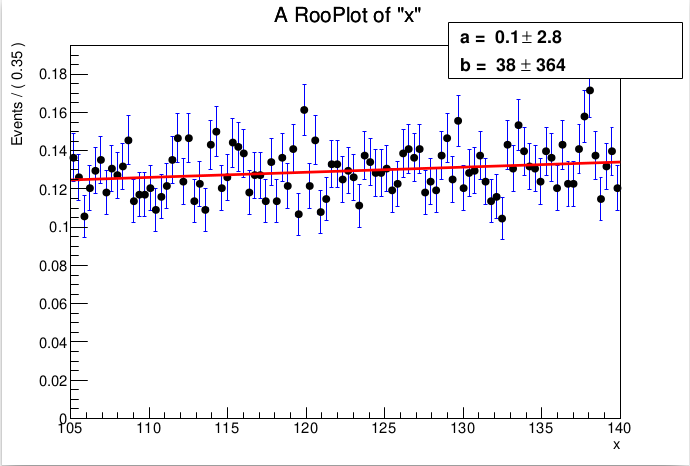
\includegraphics[width=0.8\textwidth]{background-gg.png}
			\caption[Saturn viđen u ultraljubičastom svjetlu.]{\label{sl:background-gg} Prilagodba pozadine gg $\rightarrow$ 4mu na polinom I.stupnja}
		\end{figure}
	
		Nakon što smo pronašli funkcije koje najbolje opisuju naše simulirane podatke, idući korak je stvaranje zajedničkog modela. Taj model predstavlja stvarne događaje u detektoru gdje su izmiješani i signalni i pozadinski događaji. Kada smo računali težine događaja, došli smo do zaključka da u detektoru signal uzme nekih 38 \% događaja, pozadina ZZ $\rightarrow$ 4mu 40\%, pozadina gg $\rightarrow$ 4mu 4.5\% ,a ostatak uzima proces (landau) . Naravno u stvarnosti dolazi i do drugih kanala raspada, ali njihov doprinos je zanemariv, što znači da je naš model vrlo dobar za opis realnih procesa u CMS detektoru.
		
		\begin{figure}[h!]
			\centering
			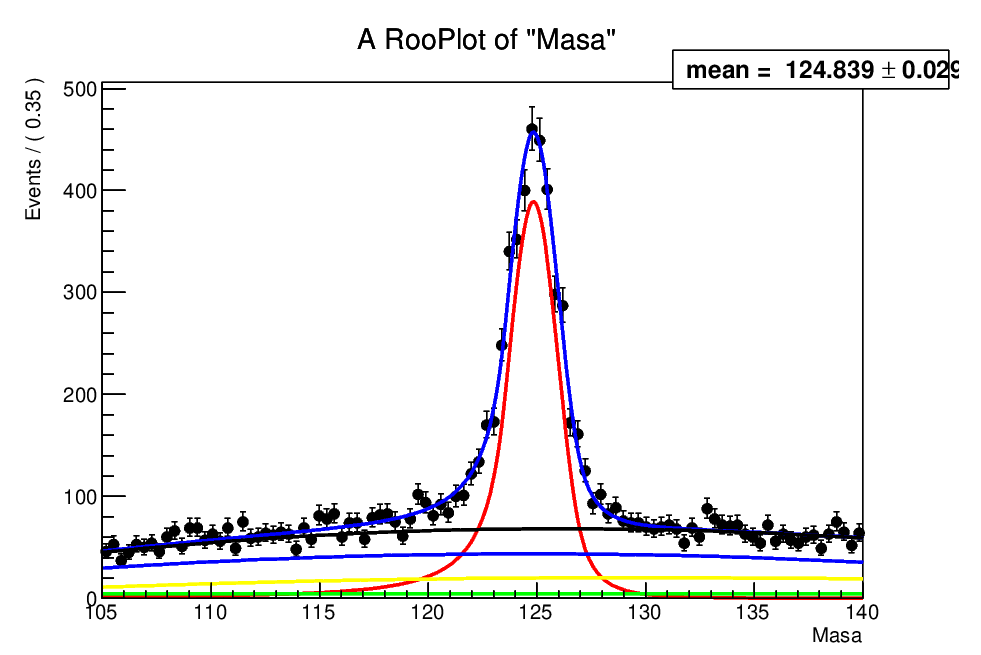
\includegraphics[width=0.8\textwidth]{simulacija-mean-fixed.png}
			\caption[Saturn viđen u ultraljubičastom svjetlu.]{\label{sl:simulacija-mean-fixed} Ukupan model s fiksnim parametrima}
		\end{figure}
		Također, interesantno je promatrati kako će se model ponašati ako pustimo da variraju svi parametri a ne samo srednja vrijednost:
		\begin{figure}[h!]
			\centering
			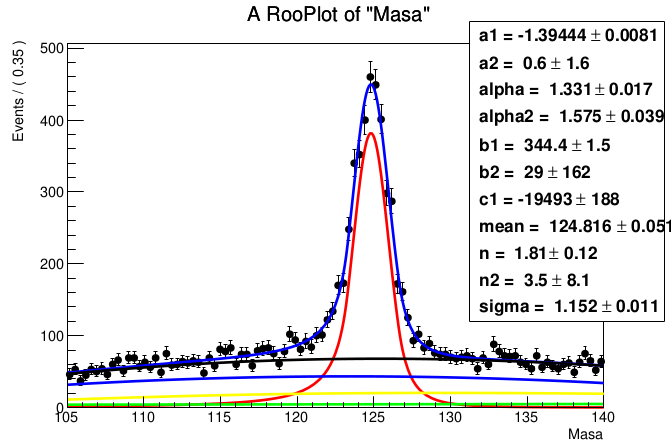
\includegraphics[width=0.8\textwidth]{simulacija-mean.png}
			\caption[Saturn viđen u ultraljubičastom svjetlu.]{\label{sl:simulacija-mean} Ukupan model s varirajućim parametrima}
		\end{figure}
		
		Kada smo se konačno uvjerili da naš model funkcija jako dobro opisuje simulirane podatke, napravili smo prilagodbu pravih podataka na takav model. Podaci na kojim to radimo su pravi podaci iz CERN-a prikupljeni iz Run-a 2 u periodu iz 2015. do 2018.godine. (//sad bih tu malo pisao koliko su se dugo podaci prikupljali i možda ubacio priču o superračunalu)
	
		\begin{figure}[h!]
			\centering
			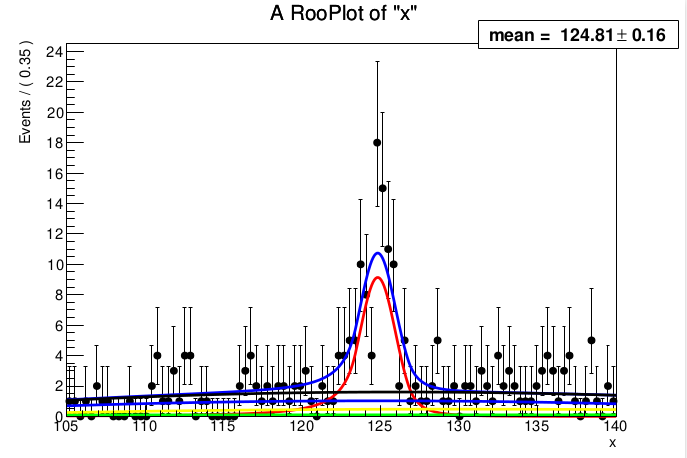
\includegraphics[width=0.8\textwidth]{final-fit-fixed1.png}
			\caption[Saturn viđen u ultraljubičastom svjetlu.]{\label{sl:final-fit-fixed} Ukupan model fitan na prave podatke s fiksnim parametrima}
		\end{figure}
		
		\begin{figure}[h!]
			\centering
			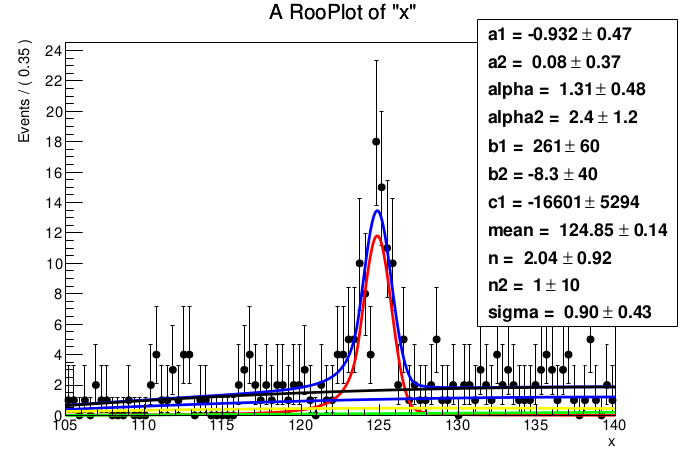
\includegraphics[width=0.8\textwidth]{final-fit1.png}
			\caption[Saturn viđen u ultraljubičastom svjetlu.]{\label{sl:final-fit} Ukupan model fitan na prave podatke s varirajućim parametrima}
		\end{figure}
		 nastavak...
		
		\newpage
		\section{Novo poglavlje}
		\subsection{Potpoglavlje}
		U tekstu opišite što se nalazi na slici. Ako slika nije vaša, onda obavezno navedite  izvor iz kojeg je preuzeta (npr. web stranica čija je puna adresa u popisu literature). Primjer je dan na slici \ref{sl:primjer}. 
		
		\begin{figure}[h!]
			\centering
			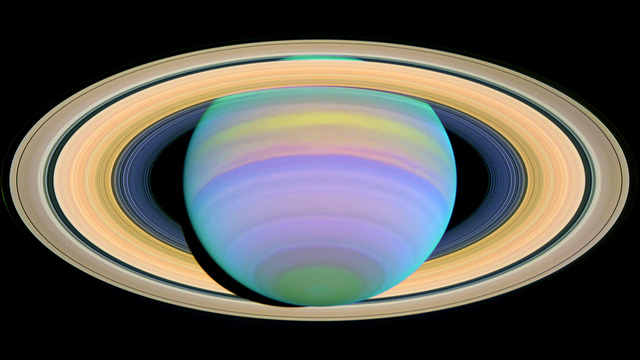
\includegraphics[width=0.8\textwidth]{slika_Saturn.png}
			\caption[Saturn viđen u ultraljubičastom svjetlu.]{\label{sl:primjer}Saturn viđen u ultraljubičastom svjetlu. Čestice u Saturnovoj atmosferi različito odbijaju svjetlost različitih valnih duljina, uzrokujući živo isticanje pojedinih područja. (slika preuzeta s \protect\url{http://hubblesite.org}~\cite{NASA}) Obratite pozornost na formatiranje.\footnotemark}
		\end{figure}
		\footnotetext{Skraćeni naslov slike unosite unutar zagrada [], a puni unutar \{\}. Za referiranje  koristite label+ref. Tekst „Slika“ i njen broj moraju biti otisnuti masnije ('bold') što je postavljeno pri učitavanju paketa caption gdje su također definirani tip ('italic') i veličina fonta 11 pt.}
		
		\begin{table}[h]
			\caption[Kapacitet i gustoća energije raznih tipova baterija.]{\label{tab:baterije}Kapacitet i gustoća energije raznih tipova baterija. Kapacitet baterije je mjera za energiju koju je moguće pohraniti i bitno ovisi o veličini baterije. To nije slučaj s gustoćom energije koja pokazuje koliko je energije moguće pohraniti po jedinici mase baterije i koja najviše ovisi o principu rada. Obratite pozornost na formatiranje.\footnotemark}
			\urediTablicu
			\begin{tabular}{?l|l|l?}
				\hlineRub
				Tip baterije & Kapacitet / (mAh) & Gustoća energije / (MJ/kg)\\ \hline
				Alkalinske AA & 2850 & 0.45 \\ \hline
				Punjive       & 1600 & 0.29 \\ \hline
				NiCd AA       & 750  & 0.15 \\ \hline
				NiMH AA       & 1100 & 0.18 \\ \hline
				Li-ion        & 1200 & 0.36 \\ \hline
				LiSOCl$_2$    &      & 1.8 \\ \hline
				Olovne        & 2000 & 0.1 \\
				\hlineRub
			\end{tabular}
		\end{table}
		\footnotetext{Tekst „Tablica“ i njen broj moraju biti otisnuti masnije ('bold') što je postavljeno pri učitavanju paketa caption. Tijelo tablice centriramo, a veličinu fonta postavljamo na 11 pt s proredom 1.5 (naredba {\color{red}\textbackslash urediTablicu}). Vanjski rubovi tablice trebaju biti debljine $1\frac{1}{2}$~pt što se može postići koristeći za vertikalne linije {\color{red}?} u specifikacijama poravnavanja, a za horizontalne naredbu {\color{red}\textbackslash hlineRub}. Debljina unutarnjih linija treba biti $\frac{3}{4}$~pt što se može postići koristeći za vertikalne linije {\color{red}|} u specifikacijama poravnavanja, a za horizontalne naredbu {\color{red}\textbackslash hline}.}
		
		Slike, tablice i grafove najbolje je postaviti na vrh ili na dno stranice. Sve oznake na njima trebaju biti na hrvatskom jeziku odnosno na jeziku kojim je pisan rad. Ukoliko to nije slučaj tekst treba zamijeniti uz pomoć programa za editiranje crteža, kao što je primjerice MS Paint. 
		
		Kod tablica, za razliku od slika, opis se nalazi iznad tablice. Primjerice pogledajte tablicu~\ref{tab:baterije}. Opis mora biti dovoljno detaljan tako da je sadržaj tablice moguće razumjeti i bez čitanja teksta rada.
		
		Kod grafikona obavezno opišite što prikazuje svaka os. U opisu navedite što predstavljaju vrijednosti, tako da se iz njega može razumjeti što graf prikazuje. Primjerice pogledajte sliku~\ref{sl:E}.
		
		\begin{figure}[t]
			\centering
			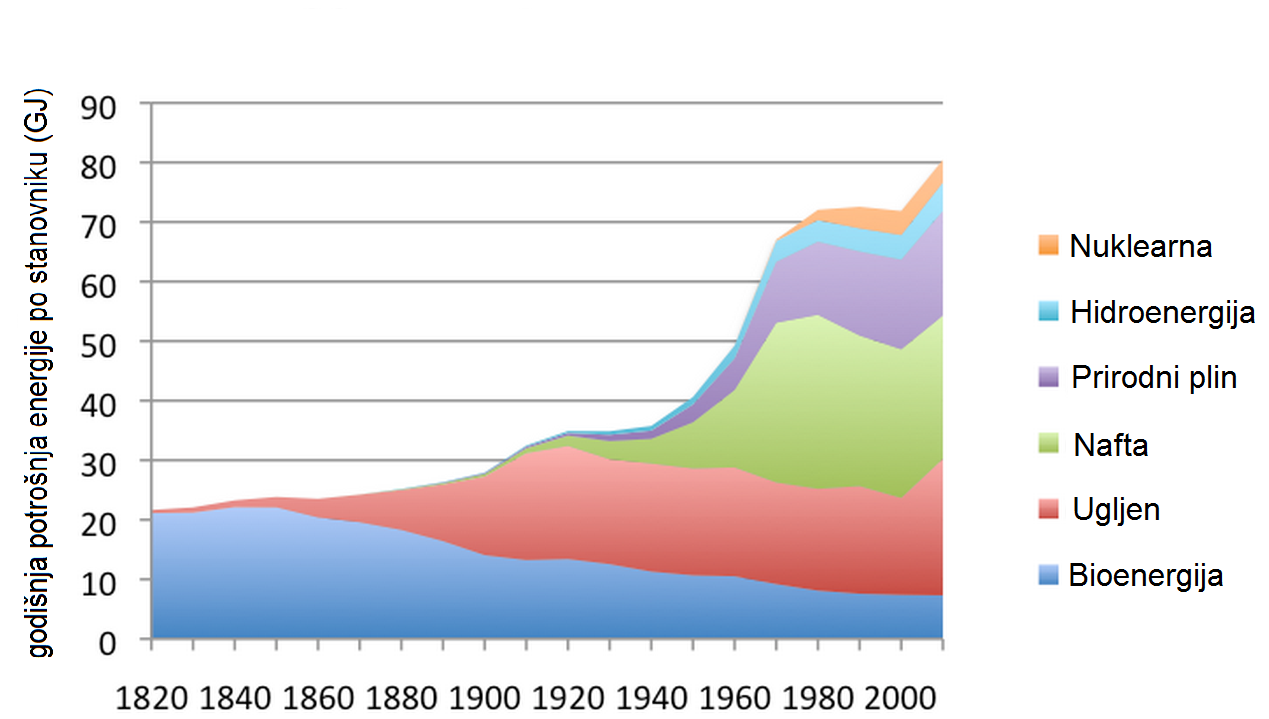
\includegraphics[width=0.72\textwidth]{slika_E-potrosnja.png}
			\caption[Prosječna godišnja potrošnja energije po stanovniku.]{\label{sl:E}Prosječna godišnja potrošnja energije po stanovniku za razne energente (y-os) izražena je kao funkcija vremena u razdoblju od 1825. godine do danas (x-os). Udio pojedinih energenata označen je različitim bojama. (graf preuzet s \protect\url{http://www.financialsense.com/}~\cite{web1})}
		\end{figure}
		
		Formule pišite u posebnom retku koristeći okruženje {\color{red}equation} koje ih numerira u skladu s brojem poglavlja. Primjerice:
		Prema II. Newtonovom zakonu potisnu silu rakete možemo odrediti iz izraza
		\begin{equation}\label{eq:F}
		\vec{F}=\frac{\Delta \vec{p}}{\Delta t}
		\end{equation}
		gdje je $\Delta p$ promjena impulsa rakete, a $\Delta t$ vrijeme u kojem je ta promjena nastala. 
		
		Radi lakšeg poravnavanja za niz jednadžbi zgodnije je koristiti okruženje {\color{red}align}, dok formule u istoj linij s tekstom unosimo unutar dijela ograničenog znakom {\color{red}\$}, tj., tekst {\color{red}\$}formula{\color{red}\$} tekst... Formule imenujte koristeći naredbu {\color{red}\textbackslash label\{{\color{black}ime}\}} te ih u tekstu pozivajte koristeći {\color{red}\textbackslash eqref\{{\color{black}ime}\}}. Primjerice, za $\Delta t \to 0$, dobivamo diferencijalni oblik jednadžbe \eqref{eq:F},
		\begin{equation}
		\vec{F}=\frac{\dif \vec{p}}{\dif t},
		\end{equation}
		pri čemu obratite pozornost na ispravno pisanje slovnih znakova\footnote{Razlikujte $\dif$ (obični tekst, operator, ime funkcije, prefiks...) i $d$ (parametar, fizikalna veličina...).} što je detaljnije objašnjeno kroz primjere u literaturi~\cite{formule}. 
		
		\newpage
		\section{Zaključak}
		Zaključak je ,,drugi najvažniji dio'' pisanog dijela rada, jer je ono što će čitatelj pogledati odmah nakon sažetka. Stoga u zaključku možete opširnije \textbf{navesti} što je sve u radu napravljeno i koje su glavne poruke. U zaključku trebate dati svoje viđenje cjelokupne tematike. To uključuje razloge za i protiv, moguća poboljšanja, daljnji rad na temi, itd. Zaključak mora biti dovoljno kratak i jasan da se samo njegovim čitanjem može steći određen uvid u mišljenje onoga tko je napisao rad. (između 200 i 400 riječi)
		
		
		\stepcounter{section} %NE brisati (broji Literaturu kao novo poglavlje)
		% UNIJETI LITERATURU NAREDBAMA \bibitem UNUTAR thebibliography
		\newpage
		{\raggedright
			\begin{thebibliography}{99}
				\bibitem{doktorat}
				T. Šćulac, \textit{Measurements of Higgs boson properties
					in the four-lepton channel in pp collisions
					at centre-of-mass energy of 13 TeV with
					the CMS detector}, 
				
				\bibitem{dokt2}
				Search for the Standard Model Higgs boson produced in
				association with a pair of top quarks and decaying into
				channel at s = 8 TeV
				with the ATLAS experiment at the LHC
				
				\bibitem{rokoplestina}
				Potencijal CMS detektora za
				potragu za Higgsovim bozonom kroz
				kanal raspada
				
				\bibitem{cernweb}
				https://home.cern/science/physics/higgs-boson
				
				\bibitem{cern-wiki}
				https://en.wikipedia.org/wiki/CERN
				
				\bibitem{cern-lhc}
				https://home.cern/science/accelerators/large-hadron-collider
				
				\bibitem{cern-tracker}
				
				\bibitem{mc-simulacije}
				https://en.wikipedia.org/wiki/Monte\textunderscore Carlo\textunderscore method
				
				\bibitem{roofit}
				https://en.wikipedia.org/wiki/ROOT
				
				\bibitem{struna}
				STRUNA, hrvatsko strukovno nazivlje,  URL: \url{http://struna.ihjj.hr/} (7. 1. 2014.).
				
				\bibitem{pr1}
				T. Cvitaš i N. Kallay, \textit{Fizičke veličine i jedinice Međunarodnog sustava}, Školska knjiga, Zagreb 1980.
				
				\bibitem{jedinice}
				\textit{Zakon o mjernim jedinicama}, Narodne novine br. 58, 1993, URL: \url{http://narodne-novine.nn.hr/clanci/sluzbeni/259051.html} (7. 1. 2014.).
				
				\bibitem{NASA}
				Hubblesite, NASA, Saturn's Rings in Ultraviolet Light
				URL: \url{http://hubblesite.org/gallery/album/solar_system} (7. 1. 2014.).
				
				\bibitem{web1}
				Tverberg, \textit{World Energy Consumption Since 1820 in Charts}, URL: \url{http://www.financialsense.com/contributors/gail-tverberg/world-energy-consumption-since-1820-in-charts} (7. 1. 2014.).
				
				\bibitem{formule}
				M. Vuković, \textit{Pisanje slovnih znakova u znanstvenim i tehničkim tekstovima}, URL: \url{http://www.akreditacija.hr/agencija/casopis/26.pdf} (prilog 1, 31. 3. 2017.).
				
				\bibitem{web2}
				N. S. Lewis, \textit{Toward Cost-Effective Solar Energy Use}, Science, 315, 798-801 (2007).
			\end{thebibliography}
		}
		
		% IZBRISATI DODATKE (appendix) AKO NE POSTOJE
		\newpage \appendix
		\section{Napomene o literaturi}
		Prilikom pozivanja na izvore u tekstu upisujemo brojeve pod kojima su ti izvori zavedeni u literaturi. Poželjno je korištenje automatskog unosa, odnosno kombinacije {\color{red}bibitem+cite} kao u ovom primjeru.
		
		Za upis knjige u literaturu koristite oblik:\\ Autori, naziv knjige, izdavač, mjesto izdanja, godina izdanja (primjer: referenca~\cite{pr1}).
		
		Za upis web stranice koristite oblik:\\ Autori stranice (ako su poznati), naziv stranice, URL, datum kada je stranica posjećena (pri\-mjeri: reference~\cite{struna,jedinice,NASA,web1,formule}).
		
		Za upis članka iz časopisa koristite oblik:\\ Autori, naziv članka, naziv časopisa, svezak, raspon stranica, godina izdanja (primjer: refe\-renca~\cite{web2}).
		
	\end{linenumbers}
\end{document}
